\section{Energieverlust von $\alpha$-Strahlung in Luft}
%kurz das ziel dieses versuchsteiles ansprechen, damit keine zwei �berschriften direkt �bereinander stehen!
%bei schwierigeren versuchen kann auch der theoretische hintergrund erl�utert werden. (mit formeln, herleitungen und erkl�rungen)
\label{sec:energieverlust}
In diesem Versuchsabschnitt soll der Energieverlust von $\alpha$-Strahlung in Luft, bei Normaldruck untersucht werden.

\subsection{Versuchsdurchf�hrung}
Da wie zuvor der Abstand zwischen dem Pr�parat und dem Detektor nicht variierbar ist, wird der Druck variiert. Die Spektroskopiekammer wird evakuiert. Dann werden der Verst�rker und der ACD so eingestellt, so dass das $^{226}$Ra-Spektrum deutlich zu erkennen ist. Da im Bereich von niedrigen Energien ein starker Untergrund vorhanden ist muss die Einstellschraube LLD am ADC so eingestellt werde, dass der Untergrund m�glichst gut raus gefiltert wird. 

\subsection{Kanal-Energie-Eichung}
Dann wird eine Kanal-Zeit-Eichung mit der Zerfallsreihe von $^{266}$Ra durchgef�hrt. Die Zerfallsreihe ist in Abb. \ref{fig:zerfall} zu sehen. Die Peaks werden �ber eine Multi-Gauss-Fit bestimmt, dieser besteht aus einer Summe von 4 Gaussverteilungen. Den so bestimmten Kan�len kann mit der Zerfallskette (Abb. \ref{fig:zerfall}) eine Energie zugeordnet werden. Diese Werte werden mit einer linearen Funktion gefittet (Gl. \ref{eqn:lin}).


\begin{figure}[H]
	\centering
  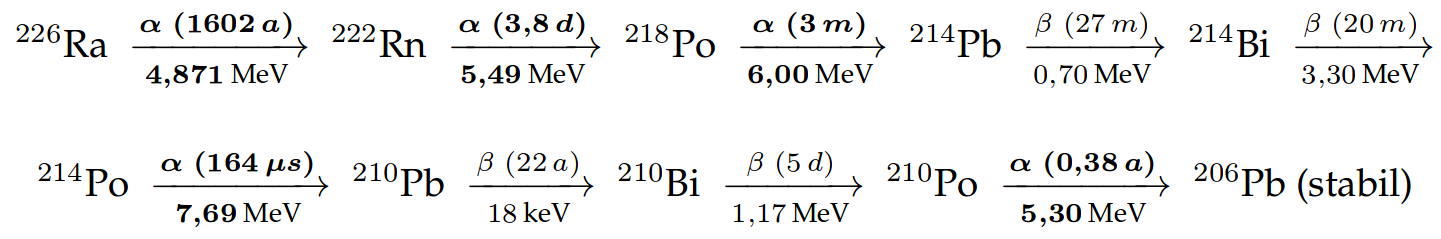
\includegraphics[scale=0.33]{zerfalls_reihe.png}
	\caption{Zerfallsreihe von $^{266}$Ra, entnommen von \cite{anleitung}}
	\label{fig:zerfall}
\end{figure}


\begin{align}
\label{eqn:lin}
E(k) = A \cdot k + B
\end{align}

Der Fehler von E(k) ergibt sich dabei nach Gl. \ref{eqn:delta_energie_kanal}.

\begin{align}
\label{eqn:delta_energie_kanal}
\Delta E = \Delta k \cdot A
\end{align}

Der Multi-Gauss-Fit ist in Abbilung \ref{fig:multi_fit} zu sehen, dabei ergaben sich die Fitparameter in Tabelle \ref{tab:multi-fit}. Die Kurve passt optisch sehr gut zu den Messdaten und das $\chi_{red}^2$ best�tigt diese Aussage mit einem Wert von 1.717.

\begin{figure}[H]
	\centering
  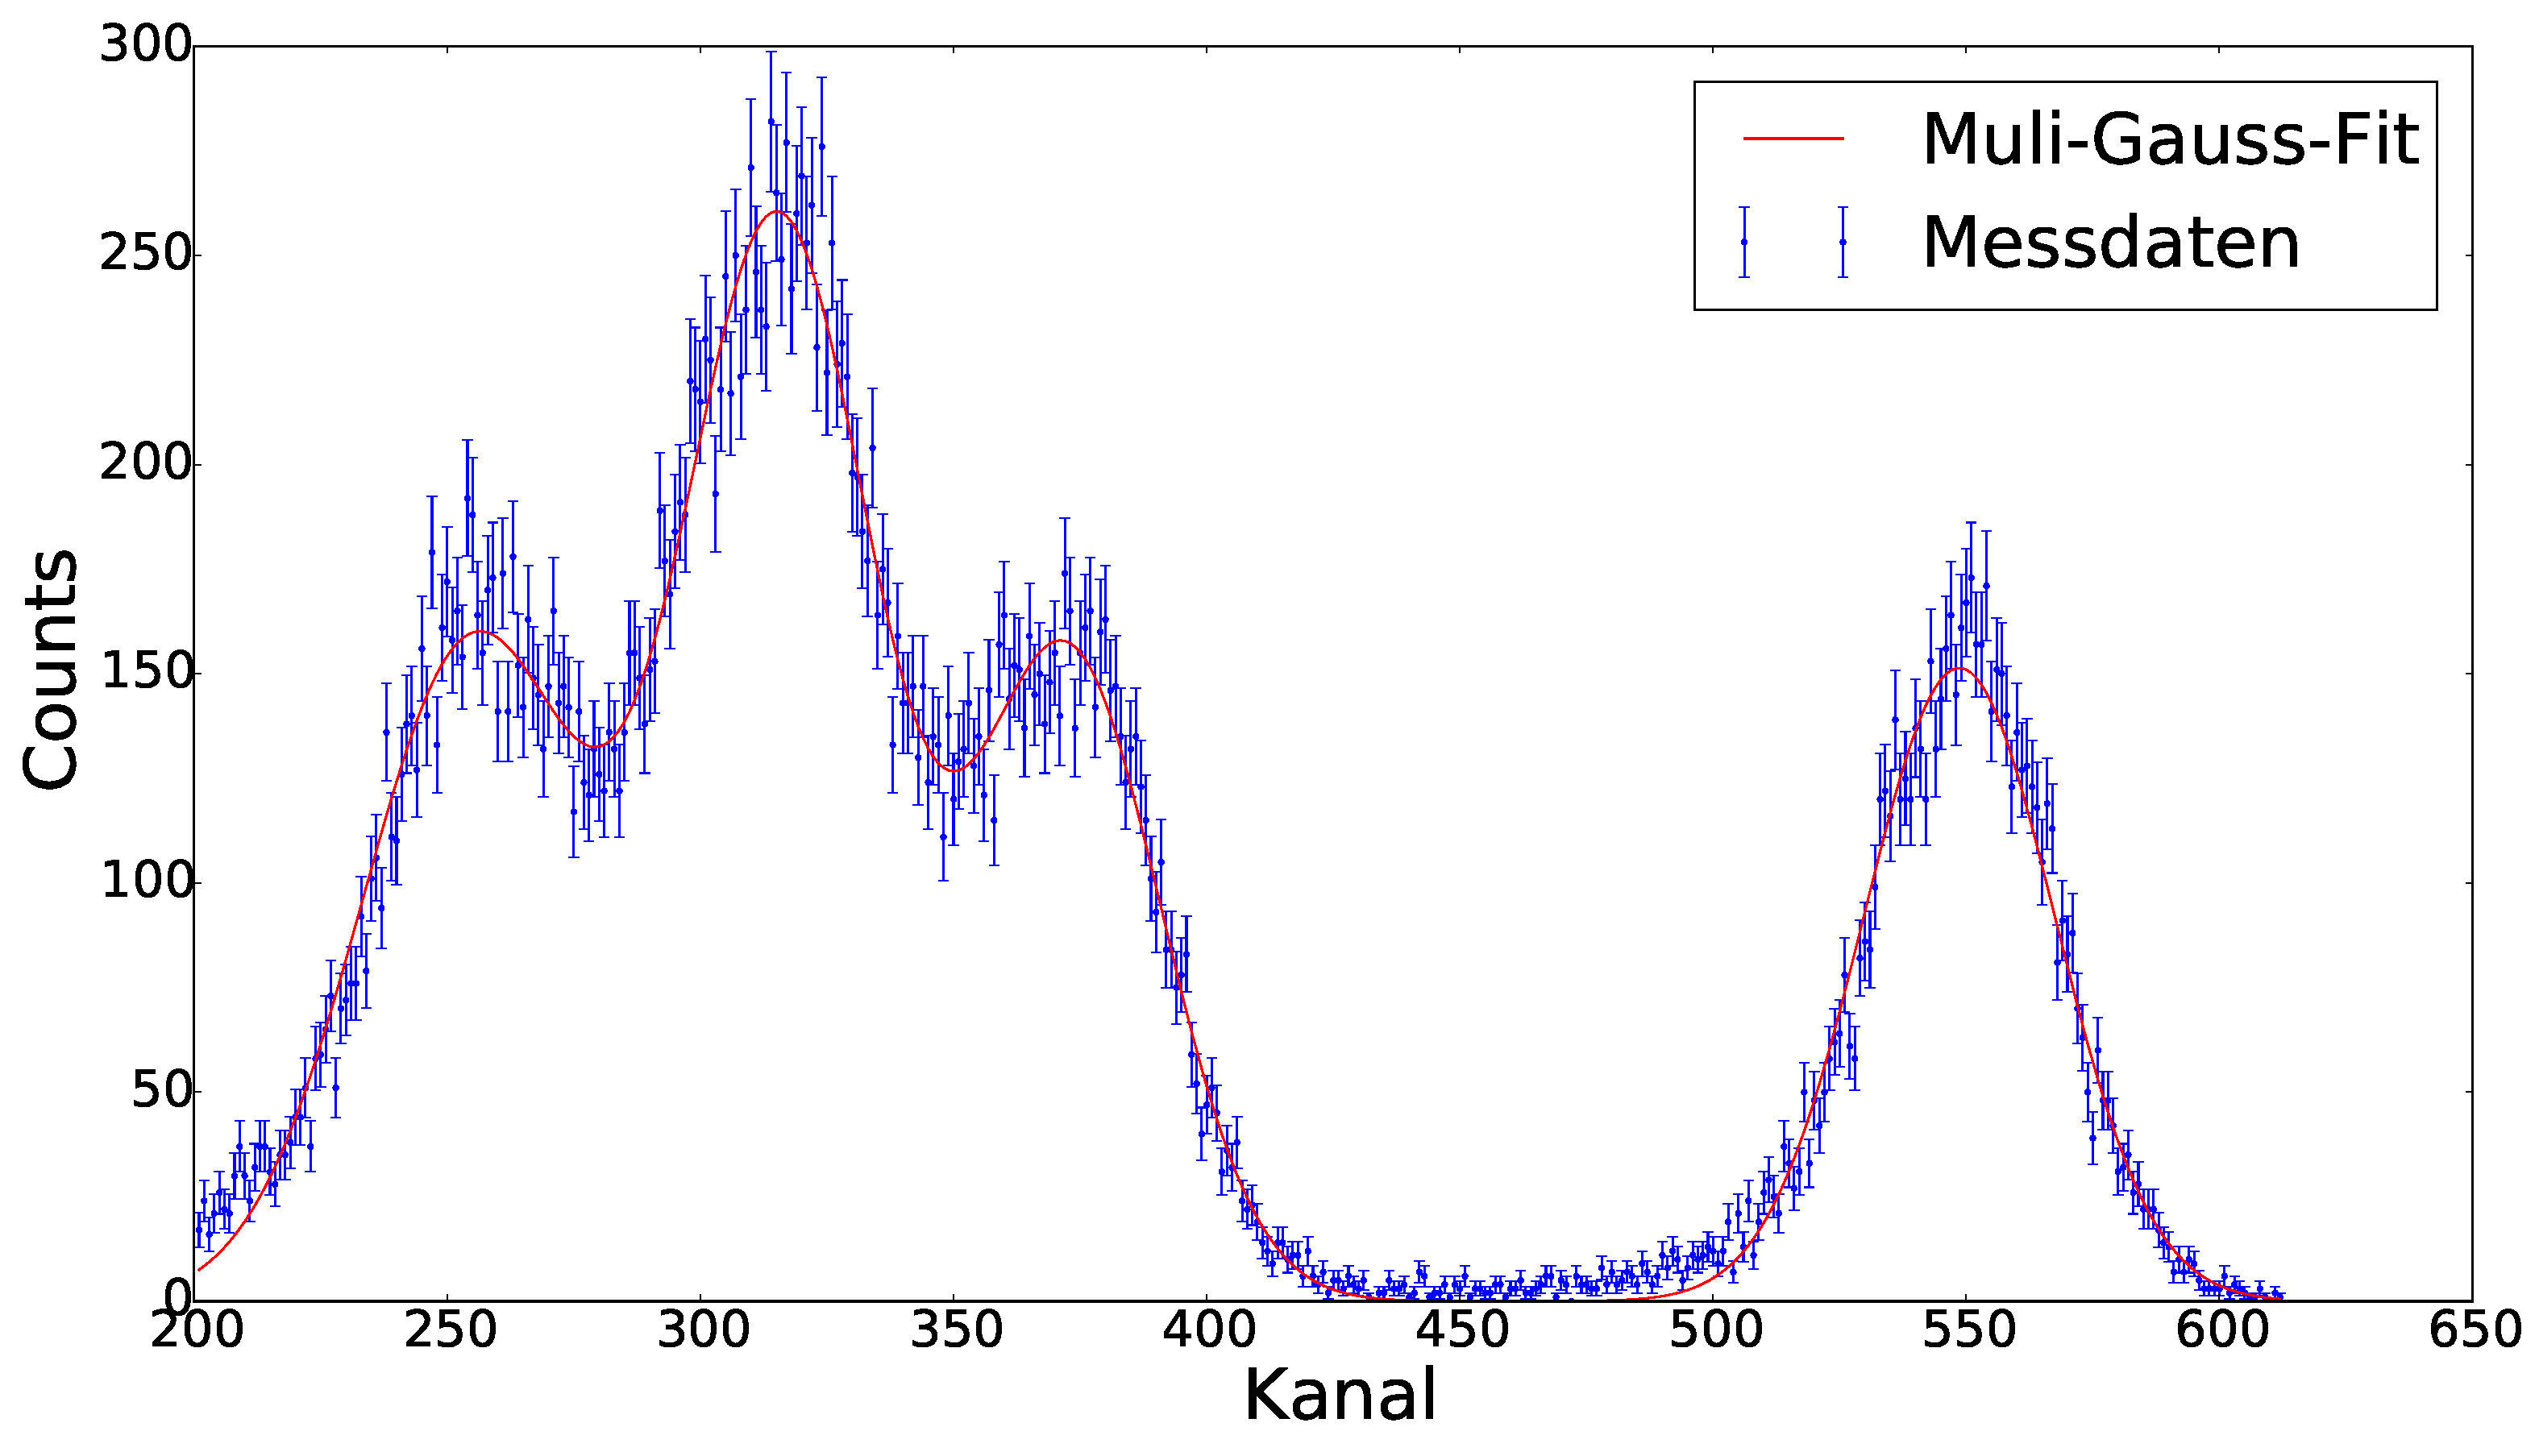
\includegraphics[scale=0.33]{multi_fit.pdf}
	\caption{Messung der des $^{226}$Ra-Zerfalls mit Multi-Gauss-Fit}
	\label{fig:multi_fit}
\end{figure}


\begin{table}[H]
\centering
\caption{Parameter des Multi-Gauss-Fits}
\label{tab:multi-fit}
\begin{tabular}{|c|c|c|c|}
\hline Gausskurve & Parameter & Wert & Fehler \\ \hline
\hline 1 & $\sigma$ & 22.0 & 0.3 \\ 
\hline  & $\mu$ & 255 & 1 \\ 
\hline  & Amplitude & 8700 & 308 \\ \hline
\hline 2 & $\sigma$ & 19.5 & 0.8 \\ 
\hline  & $\mu$ & 315.5 & 0.6 \\ 
\hline  & Amplitude & 12483 & 459 \\ \hline
\hline 3 & $\sigma$ & 18.5 & 0.5 \\ 
\hline  & $\mu$ & 372.5 & 0.8 \\ 
\hline  & Amplitude & 7156 & 243 \\ \hline
\hline 4 & $\sigma$ & 18.9 & 0.2 \\ 
\hline  & $\mu$ & 548.6 & 0.3 \\ 
\hline  & Amplitude & 7170 & 110 \\ 
\hline 
\end{tabular} 
\end{table}

Mit den Bestimmten Kan�len und den Energien ergibt sich der Plot in Abb. \ref{fig:linear_fit}, die Ergebnisse des Fits sind in Tabelle \ref{tab:linear-fit} aufgetragen. Das $\chi_{red}^2$ hat einen Wert von 0.01. Die Energie eines Kanals ist durch Gl. \ref{eqn:energie-kanal} gegeben.

\begin{figure}[H]
	\centering
  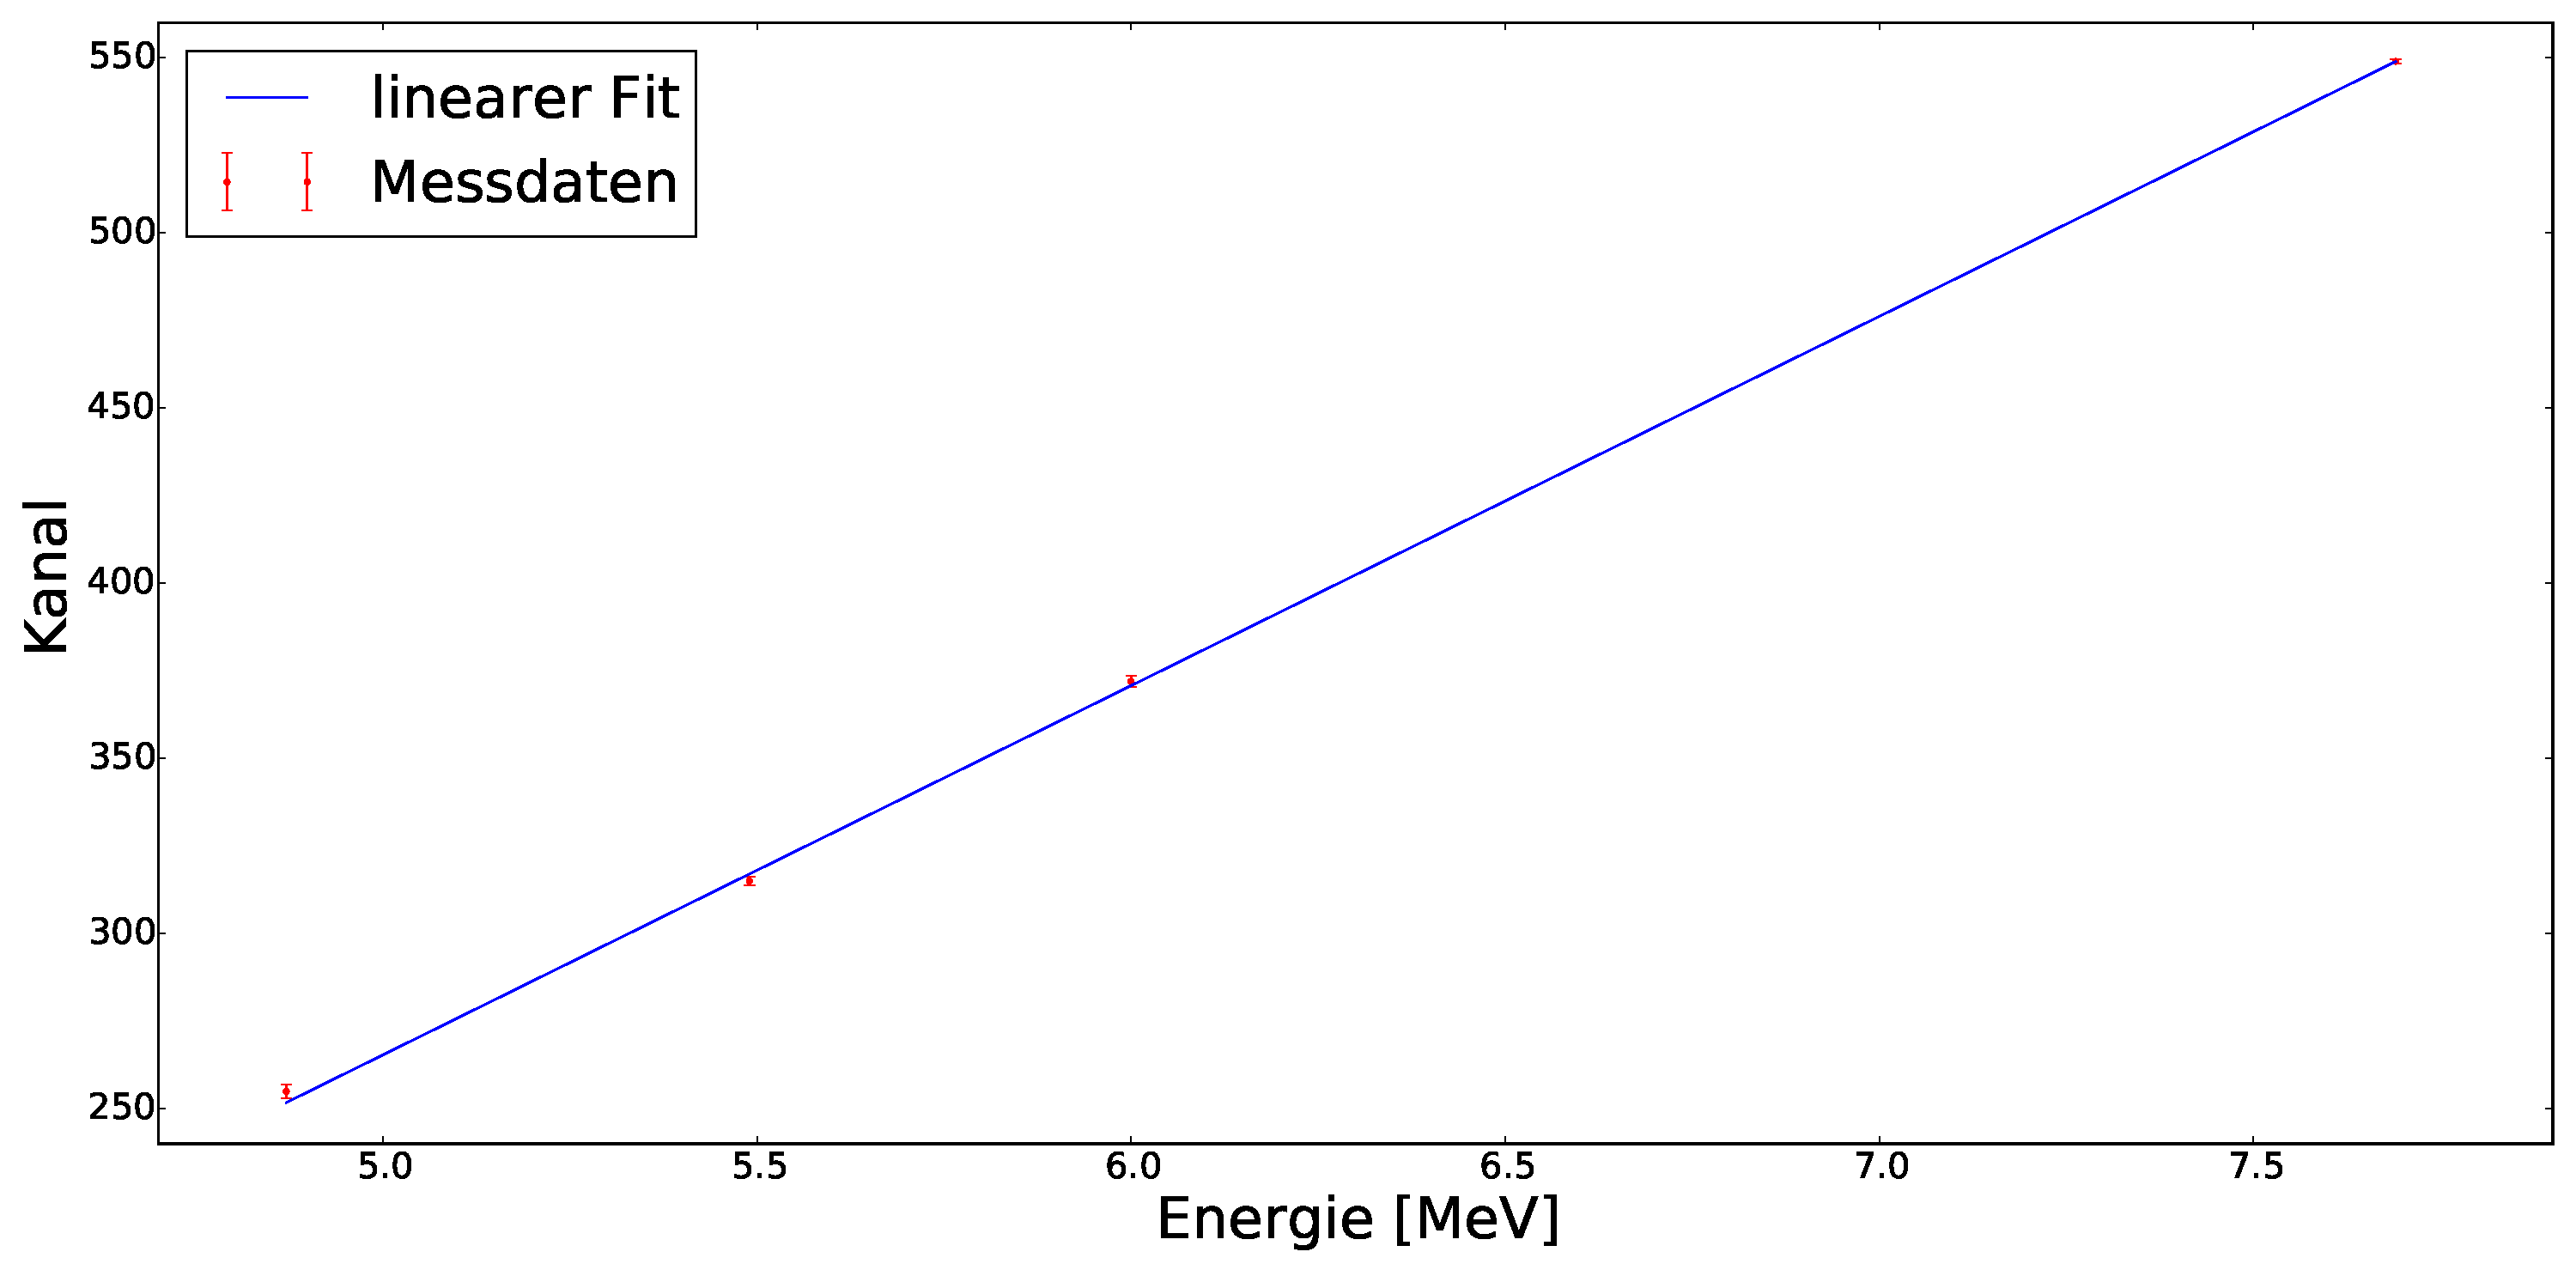
\includegraphics[scale=0.33]{linear_fit.pdf}
	\caption{Zerfallsenergien gegen die Bestimmten Kan�le mit linearem fit}
	\label{fig:linear_fit}
\end{figure}


\begin{table}[H]
\centering
\caption{Parameter des Linearen-Fits}
\label{tab:linear-fit}
\begin{tabular}{|c|c|c|}
\hline Parameter & Wert & Fehler \\ 
\hline A [MeV] & 0.0095 & 0.0001 \\ 
\hline B [MeV]& 2.46 & 0.04 \\ 
\hline 
\end{tabular} 
\end{table}

\begin{align}
\label{eqn:energie-kanal}
E(k) = (0.0095 \pm 0.0001) \cdot k + (2.46 \pm 0.04)
\end{align}


\subsection{Druckmessung}
Die Kammer wird langsam bel�ftet und Spektren im Bereich von 100 Torr bis 800 Torr in 25 Torr Schritten aufgenommen, wobei der Druck w�hrend der Messung konstant gehalten wird. Ein Bar entspricht 750.061683 Torr. Nach Gl. \ref{eqn:reich_normal} kann die Strecke mit erh�htem Druck in die Strecke unter Normaldruck umgerechnet werden. Aus den Countrates in Abh�ngigkeit des Drucks kann der absolute Energieverlust und der Energieverlust pro Wegst�ck bei Normaldruck bestimmt werden. F�r den Energieverlust pro Wegst�ck wird ein Verhalten nach Gl. \ref{eqn:reich_normal} erwartet. Die Peaks der Spektren werden wie zuvor mit einem Mulit-Gauss gefittet. Eine Messung wurde �ber eine Zeitraum von 180s durchgef�hrt.

\subsection{Energieverlust}
Der Energieverlust pro Strecke wir nach Gl. \ref{eqn:verlust} berechnet.

\begin{align}
\label{eqn:verlust}
\frac{dE}{dx} = \frac{E_1 - E_2}{x_1 - x_2}
\end{align}

Dabei ergibt sich der Fehler nach Gl. \ref{eqn:delta_verlust} bestimmt

\begin{align}
\label{eqn:delta_verlust}
\Delta \frac{dE}{dx} = \sqrt{\left( \frac{\Delta dE}{dx} \right)^2 + \left( \frac{\Delta dx \cdot dE}{dx^2} \right)^2 }
\end{align}

Die Wegdifferenz wurde mit Gleichung \ref{eqn:reich_normal} bestimmte, dabei P$_{normal}$ = 760 Torr und x$_{normal}$ = 6 cm. Die Energie wurde mit Gl. \ref{eqn:energie-kanal} bestimmt. Die Energie wurde �ber den Mittelwert bestimmt, Gl. \ref{eqn:e_mittel} der Fehler ist in Gl. \ref{eqn:delta_e_mittel} angegeben.

\begin{align}
\label{eqn:e_mittel}
\bar{E} = \frac{E_1 + E_2}{2}
\end{align}

\begin{align}
\label{eqn:delta_e_mittel}
\Delta \bar{E} = \sqrt{ \left( \frac{\Delta E_1}{2} \right)^2 + \left( \frac{\Delta E_2}{2} \right)^2}
\end{align}

Die bestimmten Peakpositonen in Abh�ngigkeit vom Druck sind in Tabelle \ref{tab:multi-fit-erg} aufgetragen. Tr�gt man nun $\frac{dE}{dx}$ gegen $dE$ auf erwartet man das von der Bethe-Bloch-Formel beschriebenen Verhalten. Die Bethe-Bloch-Formel ist in Gleichung \ref{eqn:bethe-bloch} beschrieben, da nur der Verlauf der Daten von intresse ist und nicht die Werte der einzelnen Parameter, k�nnen die Messdaten mit einem Vereinfachten Modell, Gl. \ref{eqn:bethe-bloch-einfach} gefittet werden. Dabei wird ein linearer Zusammenhang zwischen der Energie und dem Geschwindigkeitsquadrat der Teilchen angenommen ($E_{kin} \sim v^2$).

\begin{align}
\label{eqn:bethe-bloch-einfach}
\frac{dE}{dx} = \frac{A}{\beta^2} \left[ ln \left( B \cdot \beta^2 \right) - \beta^2 \right]
\end{align}

In Abb. \ref{fig:bethe_1} ist $\frac{dE}{dx}$ gegen $dE$ f�r den 4,871 MeV Peak aufgetragen, die Werte des Fits sind in Tabelle \ref{tab:bethe_fit_1} zu sehen. 

\begin{table}[H]
\centering
\caption{Fitwerte f�r den 4,871 MeV Peak nach Gl. \ref{eqn:bethe-bloch-einfach}}
\label{tab:bethe_fit_1}
\begin{tabular}{|c|c|}
\hline Parameter & Wert \\ 
\hline A & 1,8 $\pm$ 0,2 \\ 
\hline B & 3,8 $\pm$ 0,5 \\ 
\hline $\chi_{red}^2$ & 8,4 \\ 
\hline 
\end{tabular} 
\end{table}

\begin{figure}[H]
	\centering
  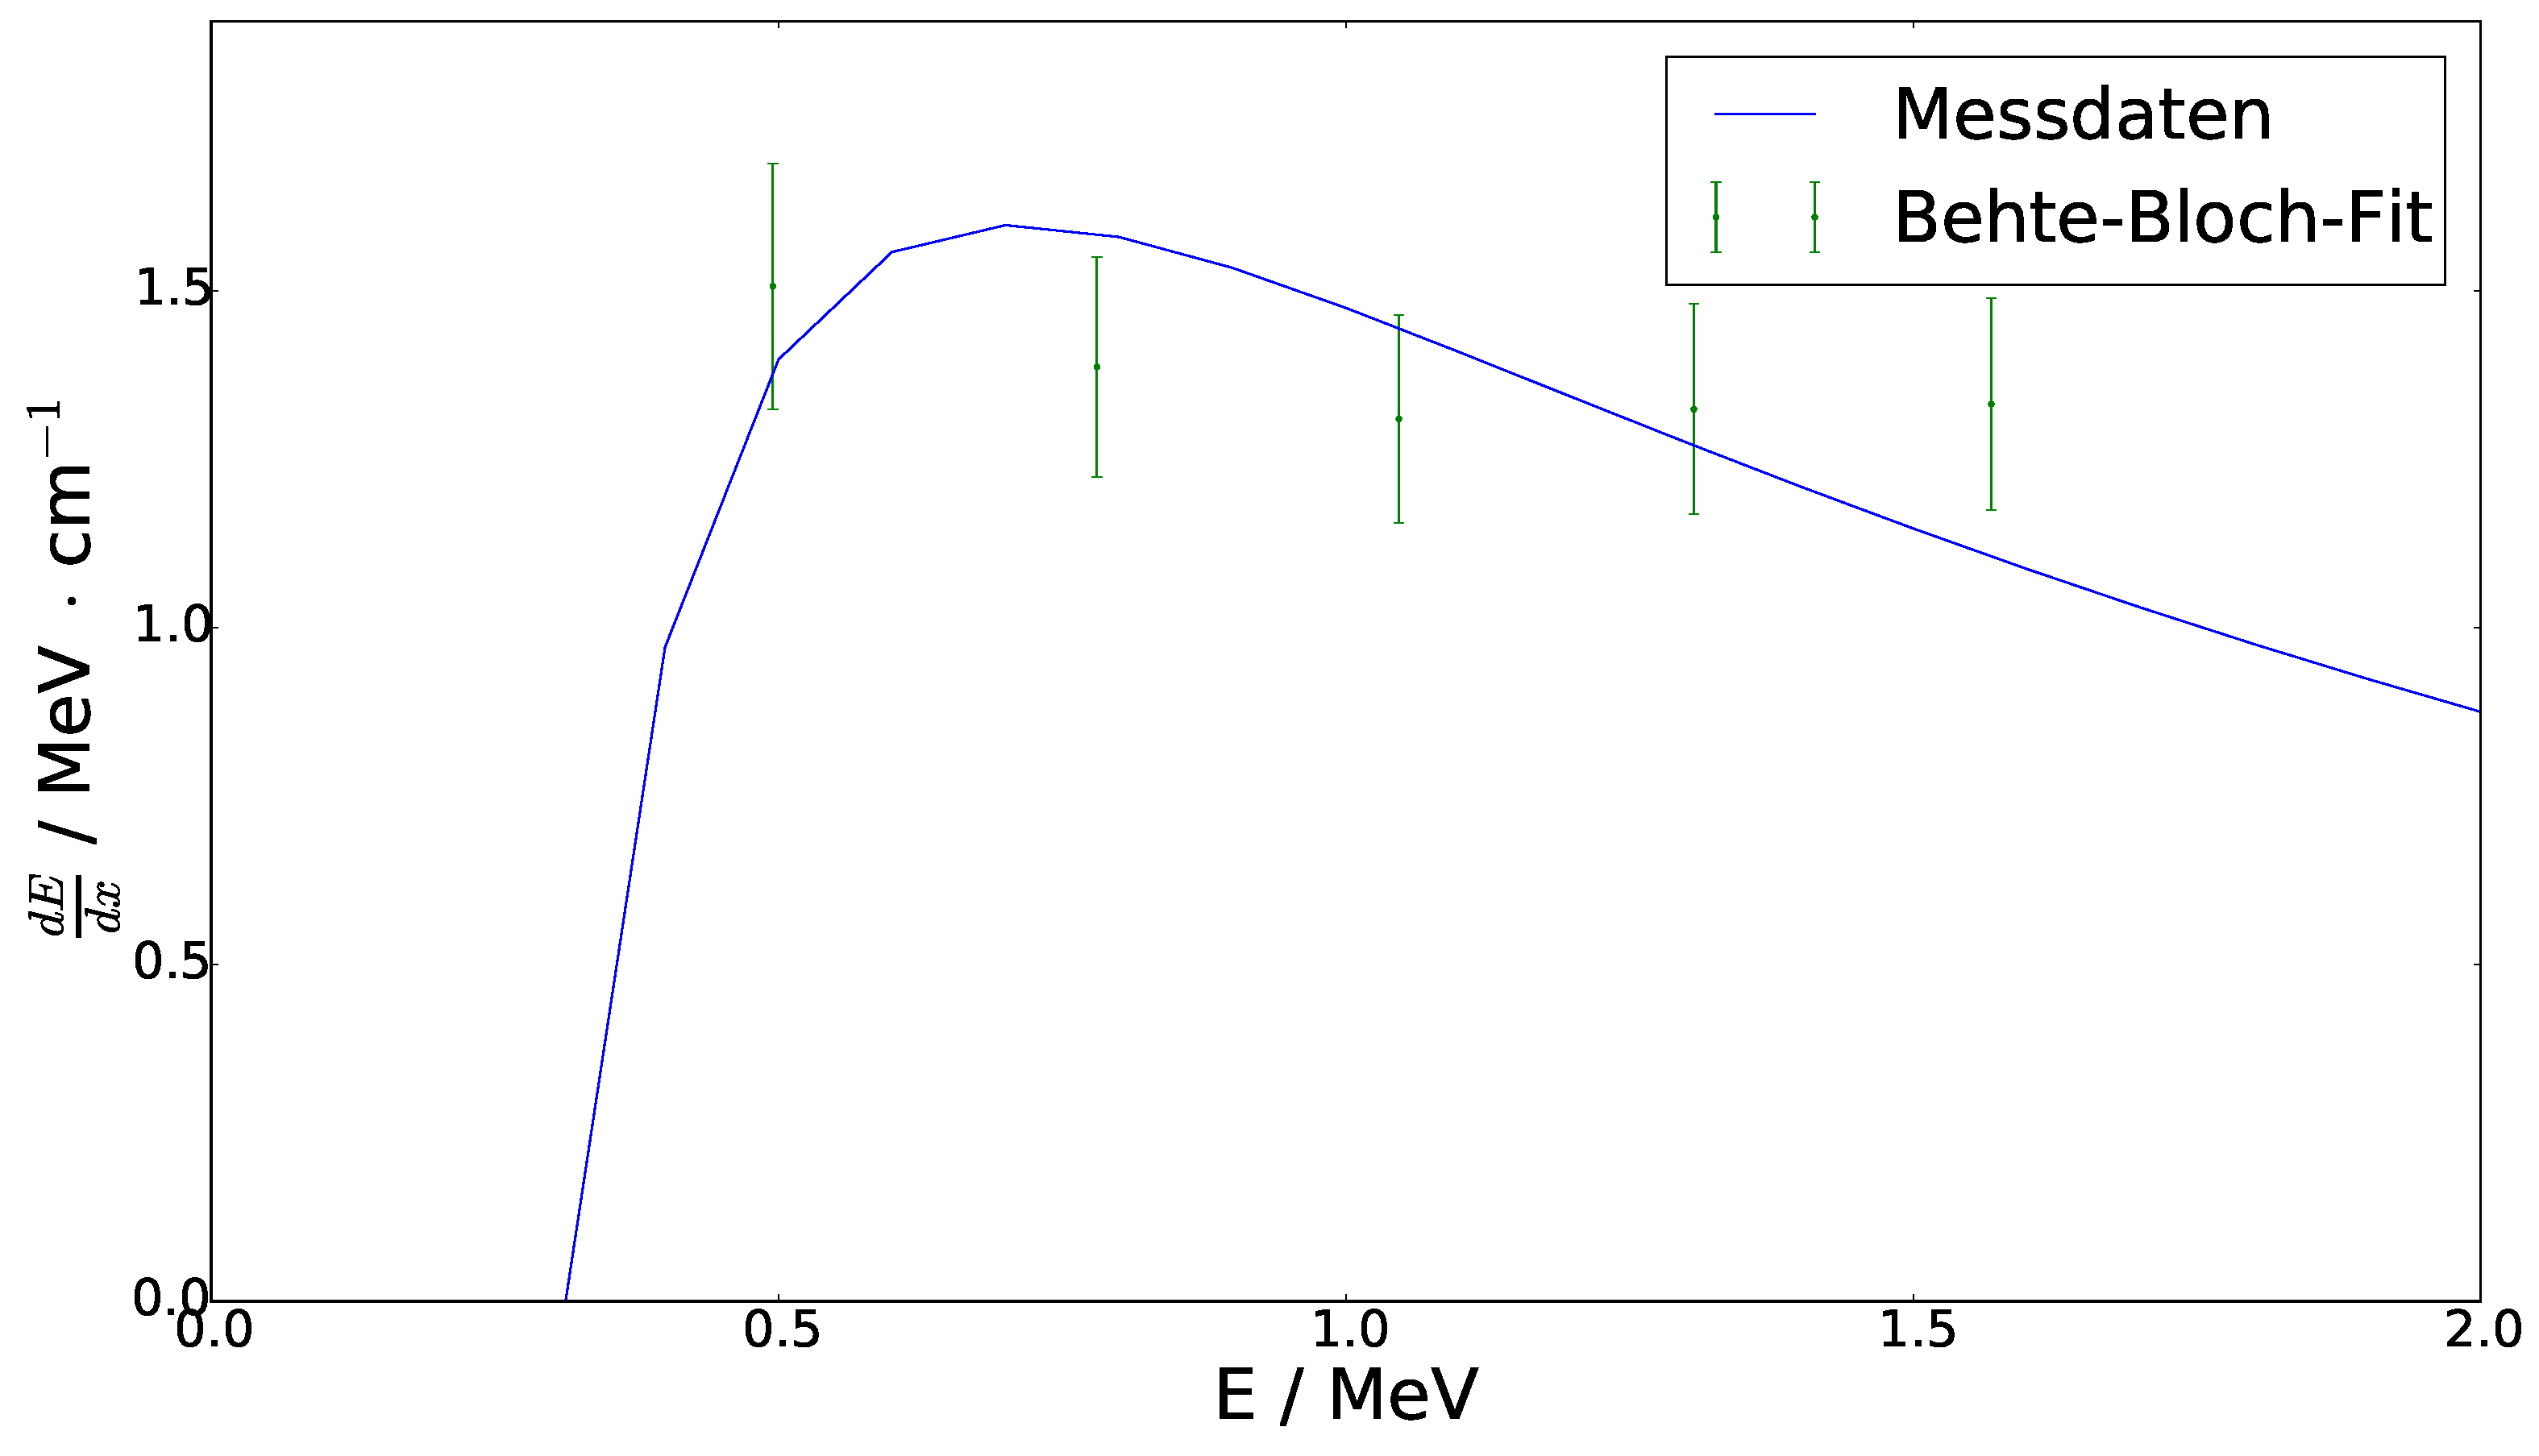
\includegraphics[scale=0.33]{bethebloch_1.pdf}
	\caption{Es ist $\frac{dE}{dx}$ gegen $dE$ aufgetragen, es wird ein Verlauf nach der Bethe-Bloch-Formel (Gl. \ref{eqn:bethe-bloch}) erwartet. Aus dem Fit mit Gl. \ref{eqn:bethe-bloch-einfach} ergibt sich ein $\chi_{red}^2$ von 8,4.}
	\label{fig:bethe_1}
\end{figure}


In Abb. \ref{fig:bethe_2} ist $\frac{dE}{dx}$ gegen $dE$ f�r den 5,49 MeV Peak aufgetragen, die Werte des Fits sind in Tabelle \ref{tab:bethe_fit_2} zu sehen. 

\begin{table}[H]
\centering
\caption{Fitwerte f�r den 5,49 MeV Peak nach Gl. \ref{eqn:bethe-bloch-einfach}}
\label{tab:bethe_fit_2}
\begin{tabular}{|c|c|}
\hline Parameter & Wert \\ 
\hline A & 2,1 $\pm$ 0,1 \\ 
\hline B & 3,2 $\pm$ 0,2 \\ 
\hline $\chi_{red}^2$ & 13,4 \\ 
\hline 
\end{tabular} 
\end{table}

\begin{figure}[H]
	\centering
  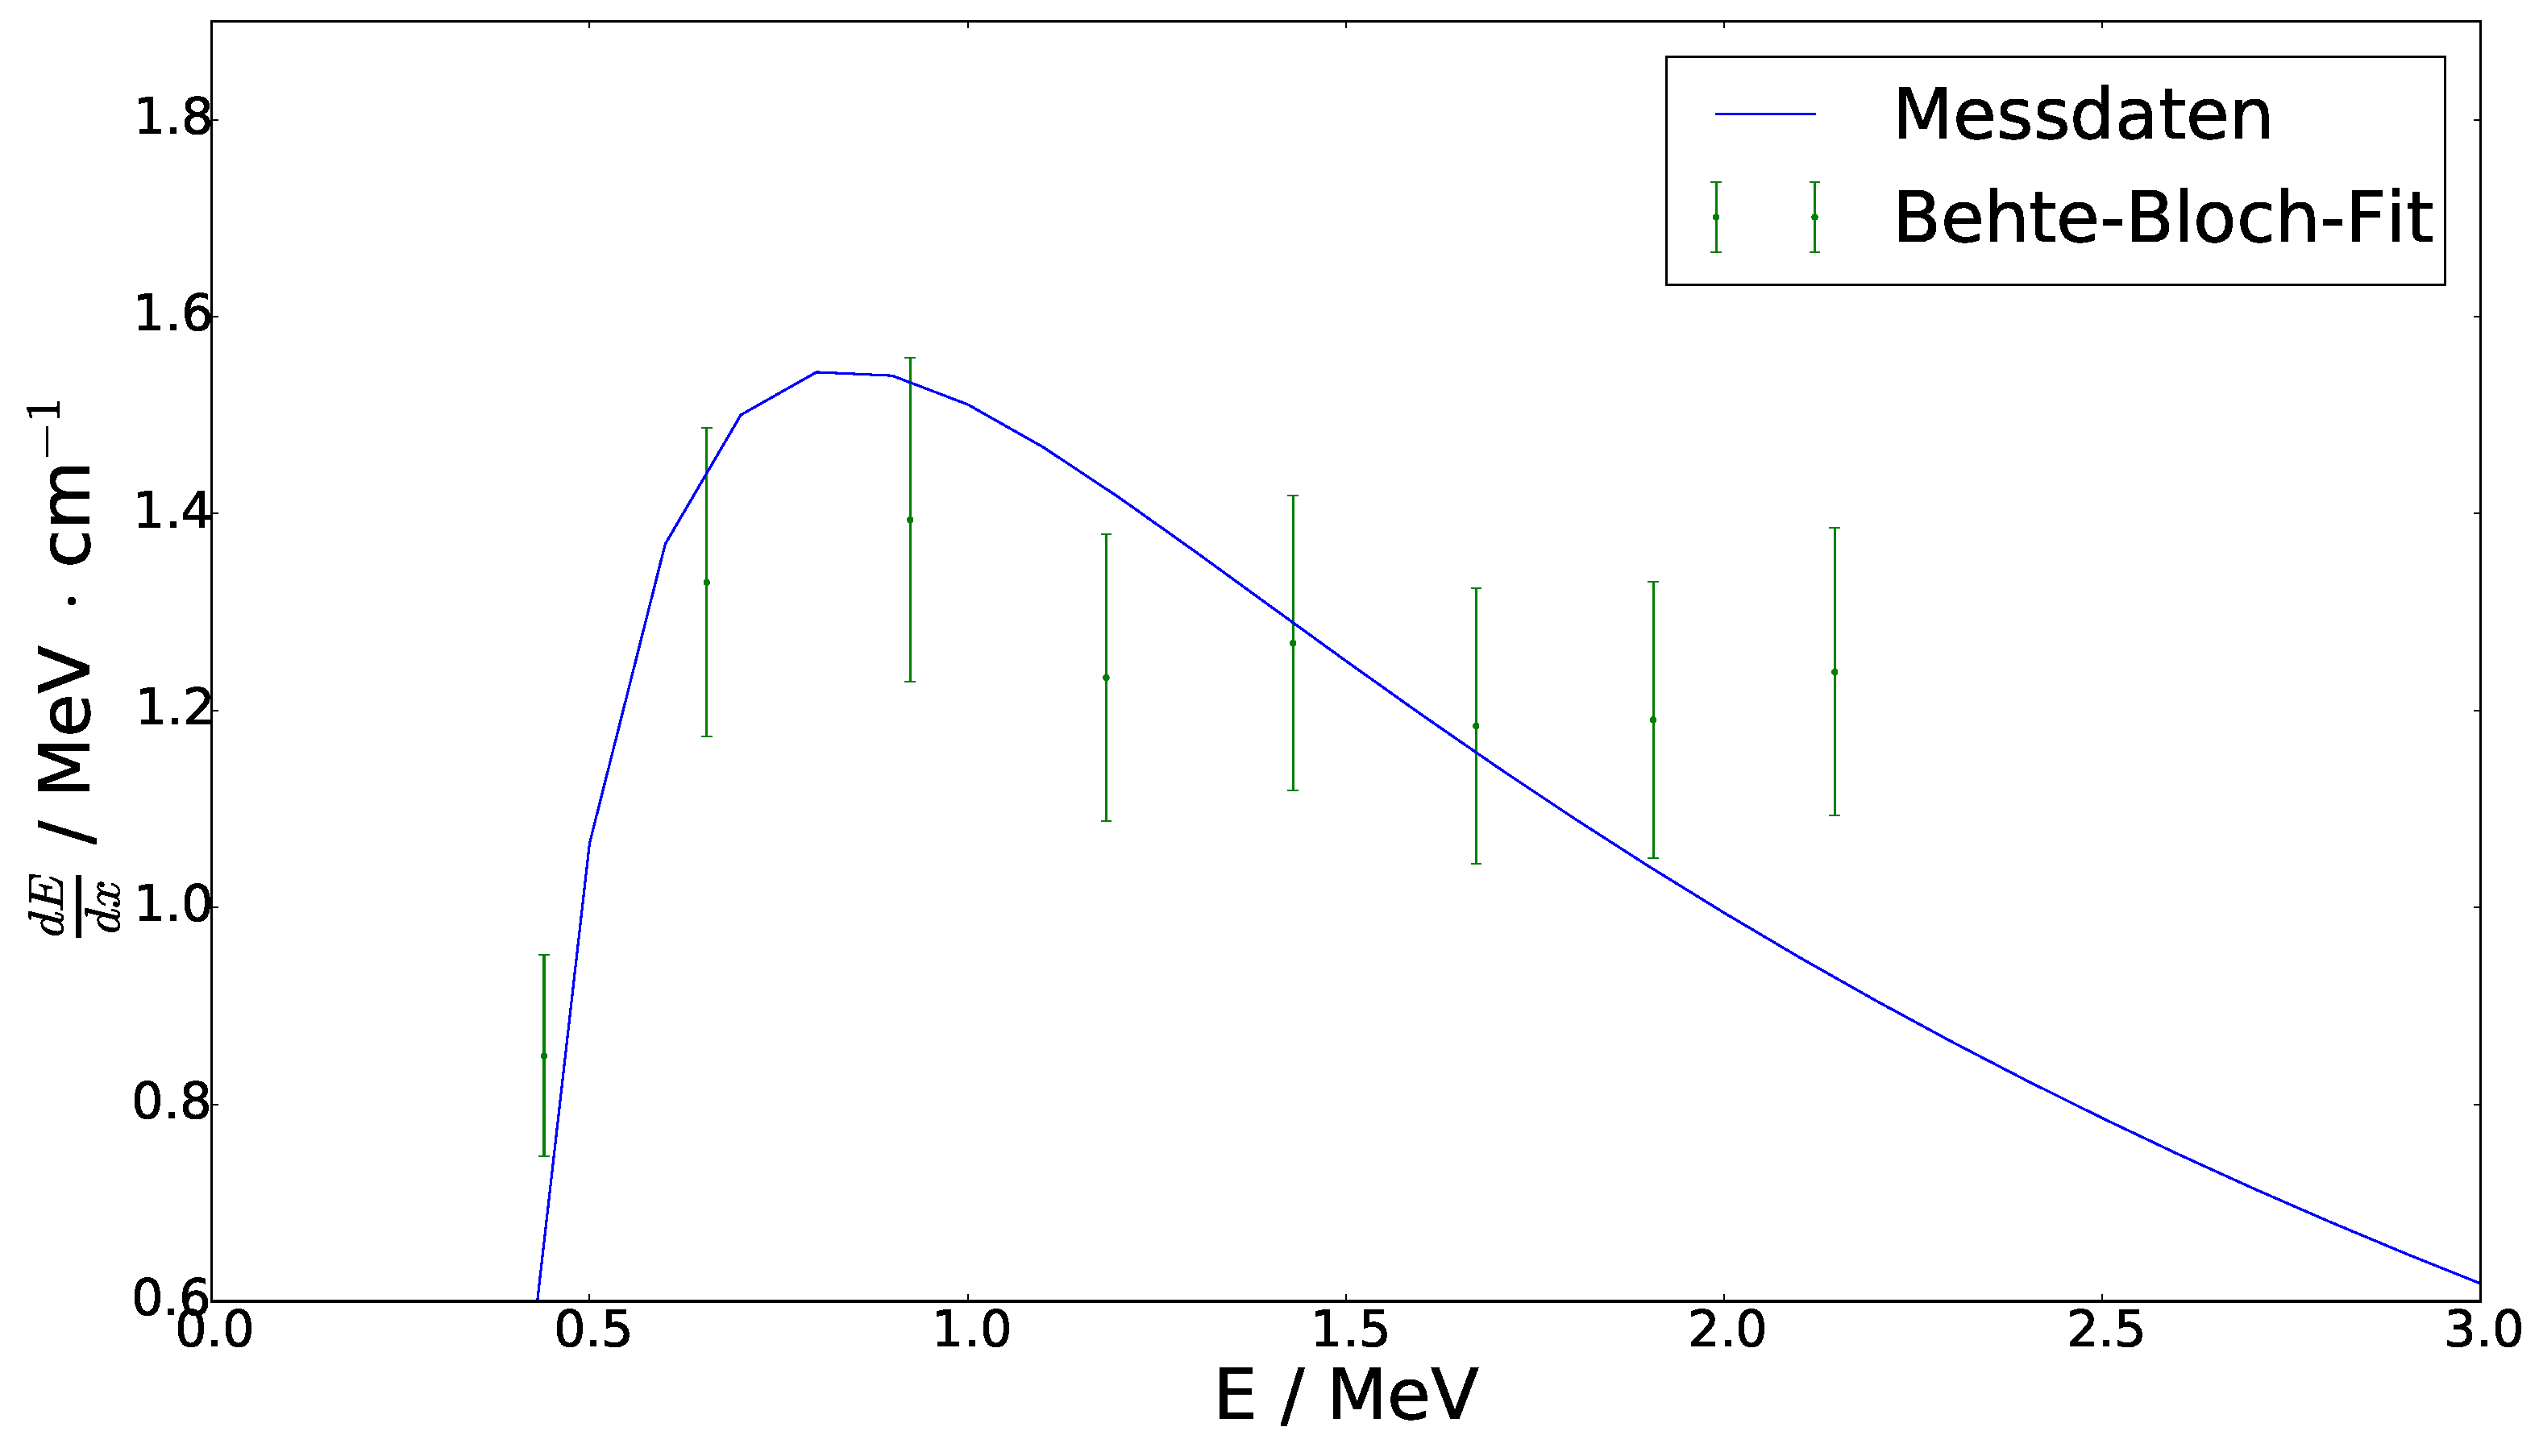
\includegraphics[scale=0.33]{bethebloch_2.pdf}
	\caption{Es ist $\frac{dE}{dx}$ gegen $dE$, f�r den 5,49 MeV Peak aufgetragen, es wird ein Verlauf nach der Bethe-Bloch-Formel (Gl. \ref{eqn:bethe-bloch}) erwartet. Aus dem Fit mit Gl. \ref{eqn:bethe-bloch-einfach} ergibt sich ein $\chi_{red}^2$ von 13,4.}
	\label{fig:bethe_2}
\end{figure}




In Abb. \ref{fig:bethe_3} ist $\frac{dE}{dx}$ gegen $dE$ f�r den 6 MeV Peak aufgetragen, die Werte des Fits sind in Tabelle \ref{tab:bethe_fit_3} zu sehen. 

\begin{table}[H]
\centering
\caption{Fitwerte f�r den 6 MeV Peak nach Gl. \ref{eqn:bethe-bloch-einfach}}
\label{tab:bethe_fit_3}
\begin{tabular}{|c|c|}
\hline Parameter & Wert \\ 
\hline A & 2,0 $\pm$ 0,1 \\ 
\hline B & 3,5 $\pm$ 0,2 \\ 
\hline $\chi_{red}^2$ & 17,5 \\ 
\hline 
\end{tabular} 
\end{table}

\begin{figure}[H]
	\centering
  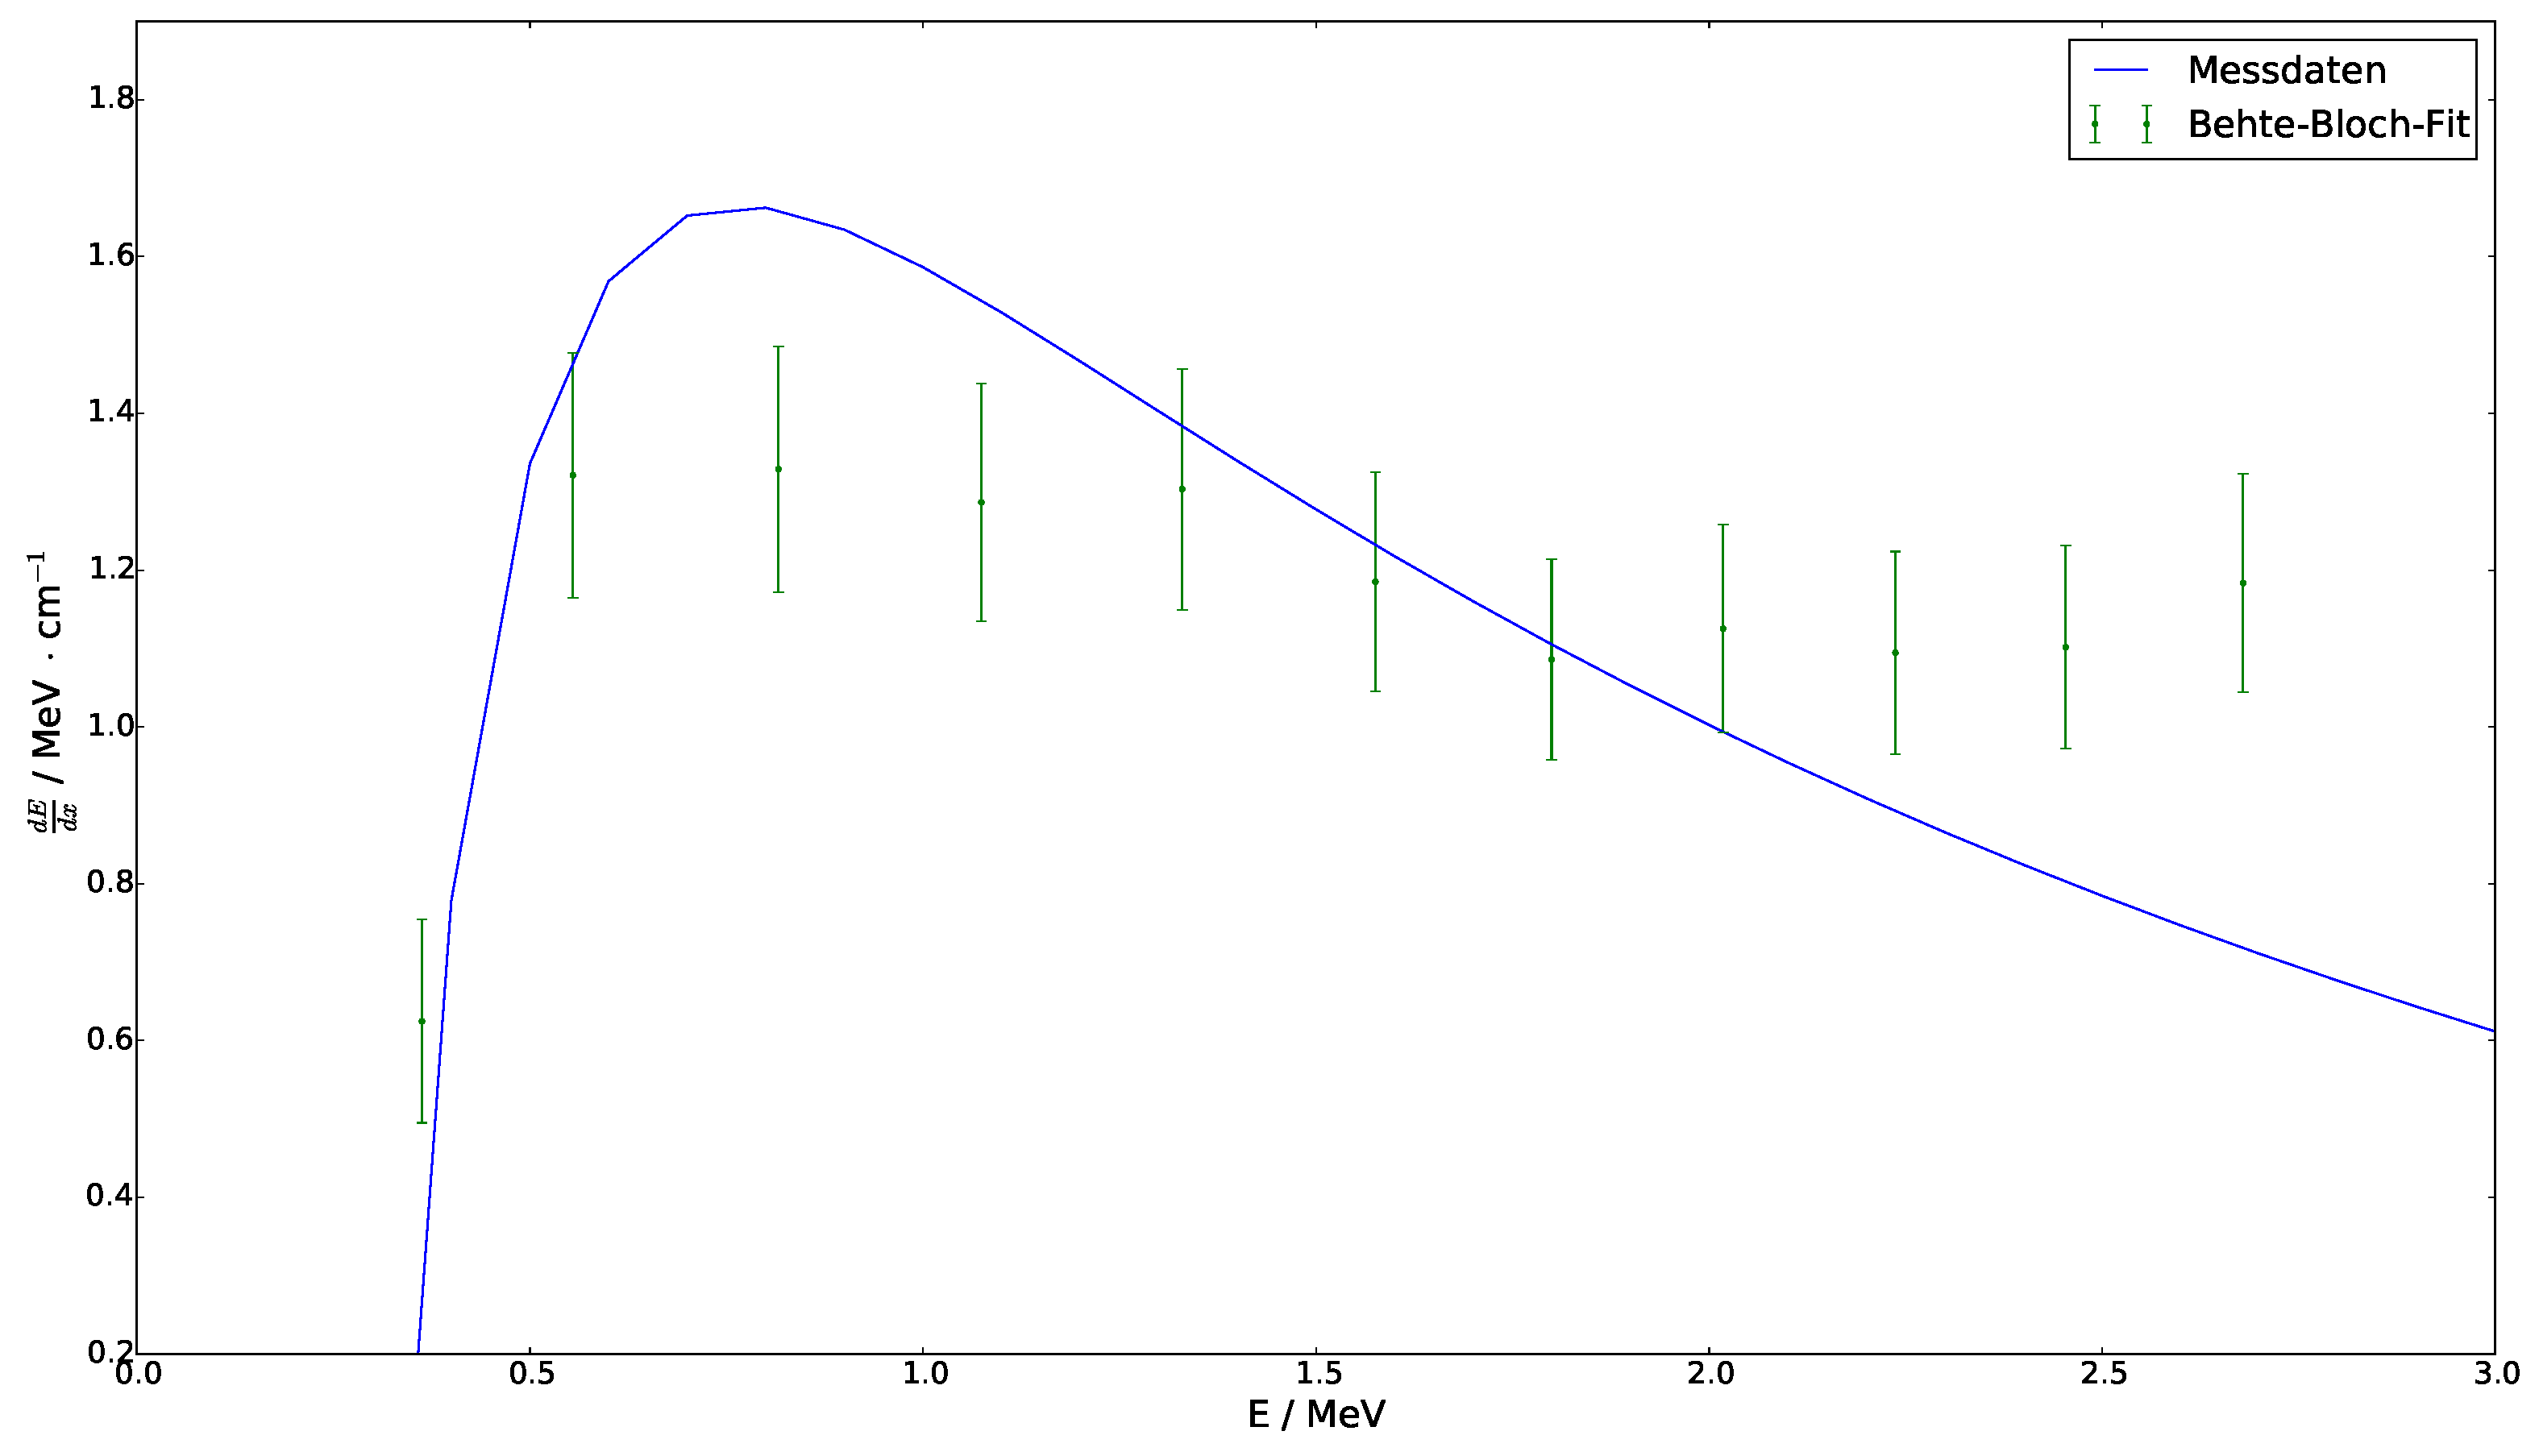
\includegraphics[scale=0.33]{bethebloch_3.pdf}
	\caption{Es ist $\frac{dE}{dx}$ gegen $dE$, f�r den 6 MeV Peak aufgetragen, es wird ein Verlauf nach der Bethe-Bloch-Formel (Gl. \ref{eqn:bethe-bloch}) erwartet. Aus dem Fit mit Gl. \ref{eqn:bethe-bloch-einfach} ergibt sich ein $\chi_{red}^2$ von 17,5.}
	\label{fig:bethe_3}
\end{figure}



In Abb. \ref{fig:bethe_4} ist $\frac{dE}{dx}$ gegen $dE$ f�r den 7,69 MeV Peak aufgetragen, die Werte des Fits sind in Tabelle \ref{tab:bethe_fit_4} zu sehen. 

\begin{table}[H]
\centering
\caption{Fitwerte f�r den 7,69 MeV Peak nach Gl. \ref{eqn:bethe-bloch-einfach}}
\label{tab:bethe_fit_4}
\begin{tabular}{|c|c|}
\hline Parameter & Wert \\ 
\hline A & 2,3 $\pm$ 0,2 \\ 
\hline B & 3,2 $\pm$ 0,3 \\ 
\hline $\chi_{red}^2$ & 30,9 \\ 
\hline 
\end{tabular} 
\end{table}

\begin{figure}[H]
	\centering
  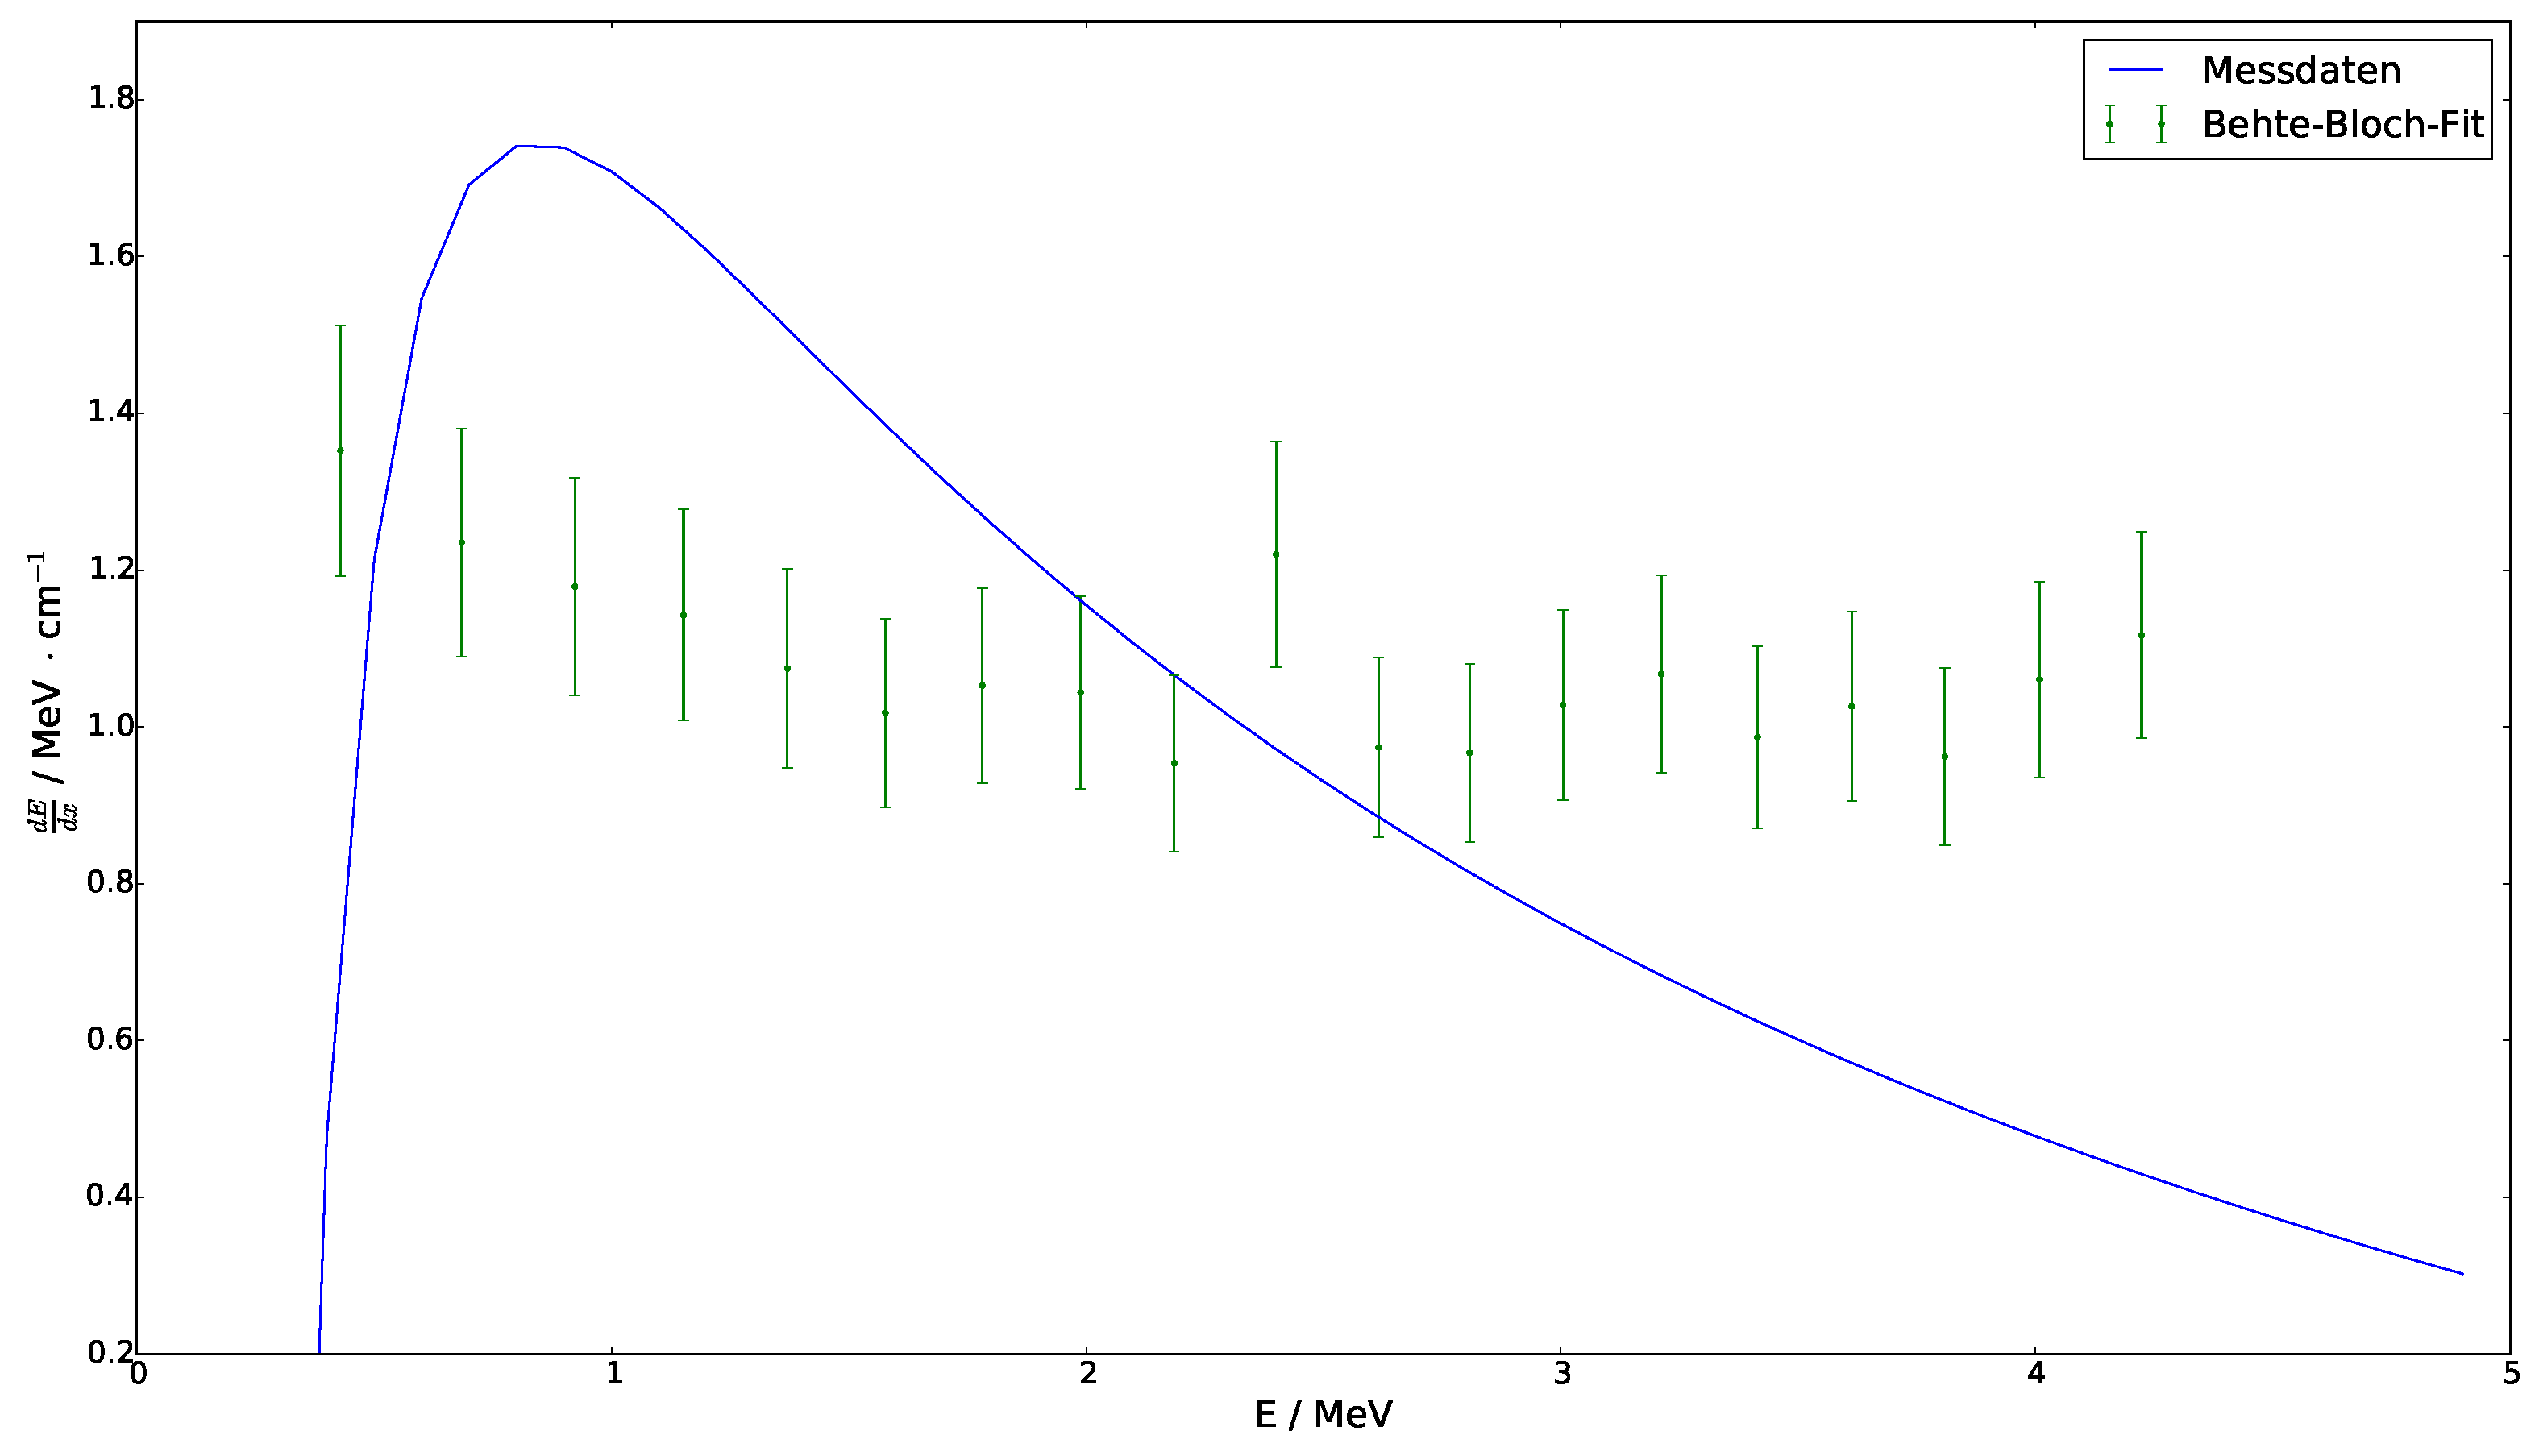
\includegraphics[scale=0.33]{bethebloch_4.pdf}
	\caption{Es ist $\frac{dE}{dx}$ gegen $dE$, f�r den 7,69 MeV Peak aufgetragen, es wird ein Verlauf nach der Bethe-Bloch-Formel (Gl. \ref{eqn:bethe-bloch}) erwartet. Aus dem Fit mit Gl. \ref{eqn:bethe-bloch-einfach} ergibt sich ein $\chi_{red}^2$ von 30,9.}
	\label{fig:bethe_4}
\end{figure}



Das $\chi_{red}^2$ liegt bei allen Fits weit oberhalb von 1, dabei f�llt auf, dass die ersten Werte besser an an die Behte-Bloch-Kurve passen, ab einem bestimmten Energiewert, steigt $\frac{dE}{dx}$ bei allen Peaks. Der Energiewert, ab dem $\frac{dE}{dx}$ steigt, ist bei jedem Peak anders, weshalb ein systematische Fehler ab einer bestimmten Messung ausgeschlossen werden kann. Die Quelle des Fehlers ist Unbekannt. Wie sich in Abschnitt \ref{subsec:bragg} zeigt, ist der Verlauf der Bragg-Kurven bei allen Messungen  wie erwartet.

\subsection{Bragg-Kurve}
\label{subsec:bragg}
Tr�gt man $\frac{dE}{dx}$ gegen die zur�ckgelgete Strecke auf, so erwartet man ein Verhalten wie in Abb. \ref{fig:braggkurve}.

In Abb. \ref{fig:bragg_1} ist f�r den 4,871 MeV Peak $\frac{dE}{dx}$ gegen $x$ zusehen.

\begin{figure}[H]
	\centering
  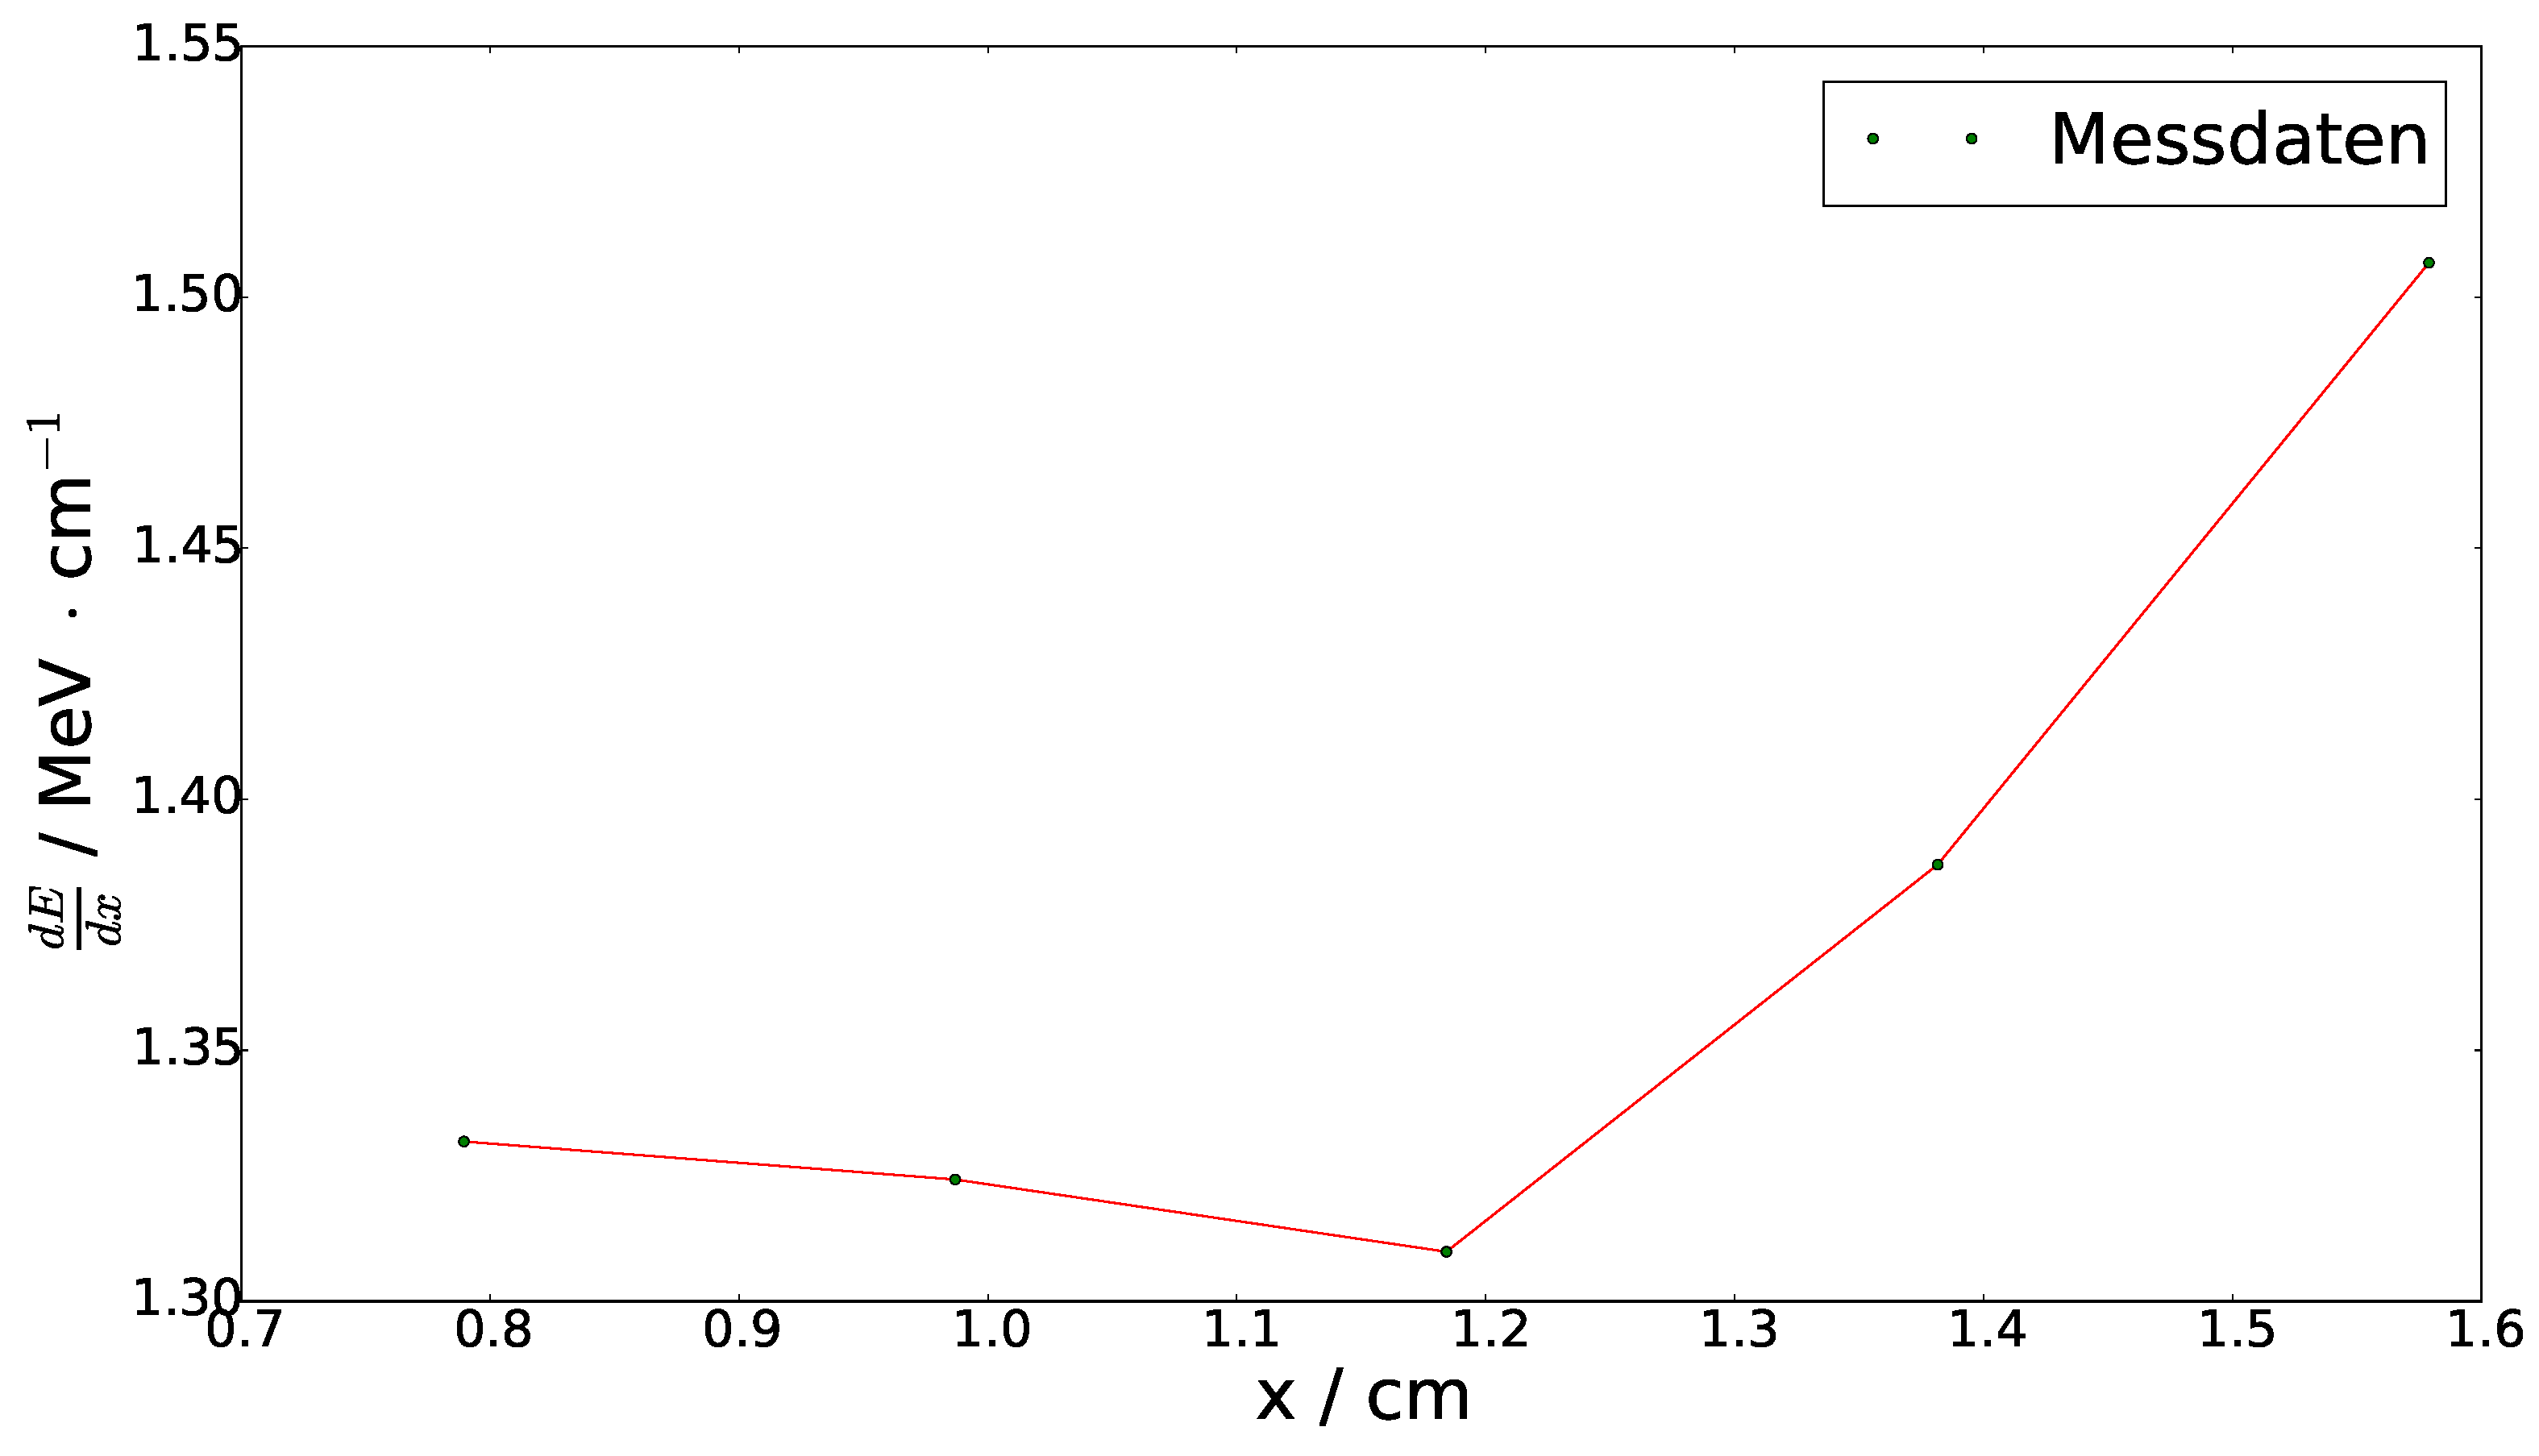
\includegraphics[scale=0.33]{bragg_kurve_1.pdf}
	\caption{$\frac{dE}{dx}$ gegen $x$ Aufgetragen , es ist deutlich der Anfang des Braggpeaks zu sehen}
	\label{fig:bragg_1}
\end{figure}

\noindent
In Abb. \ref{fig:bragg_2} ist f�r den 5,49 MeV Peak $\frac{dE}{dx}$ gegen $x$ zusehen.

\begin{figure}[H]
	\centering
  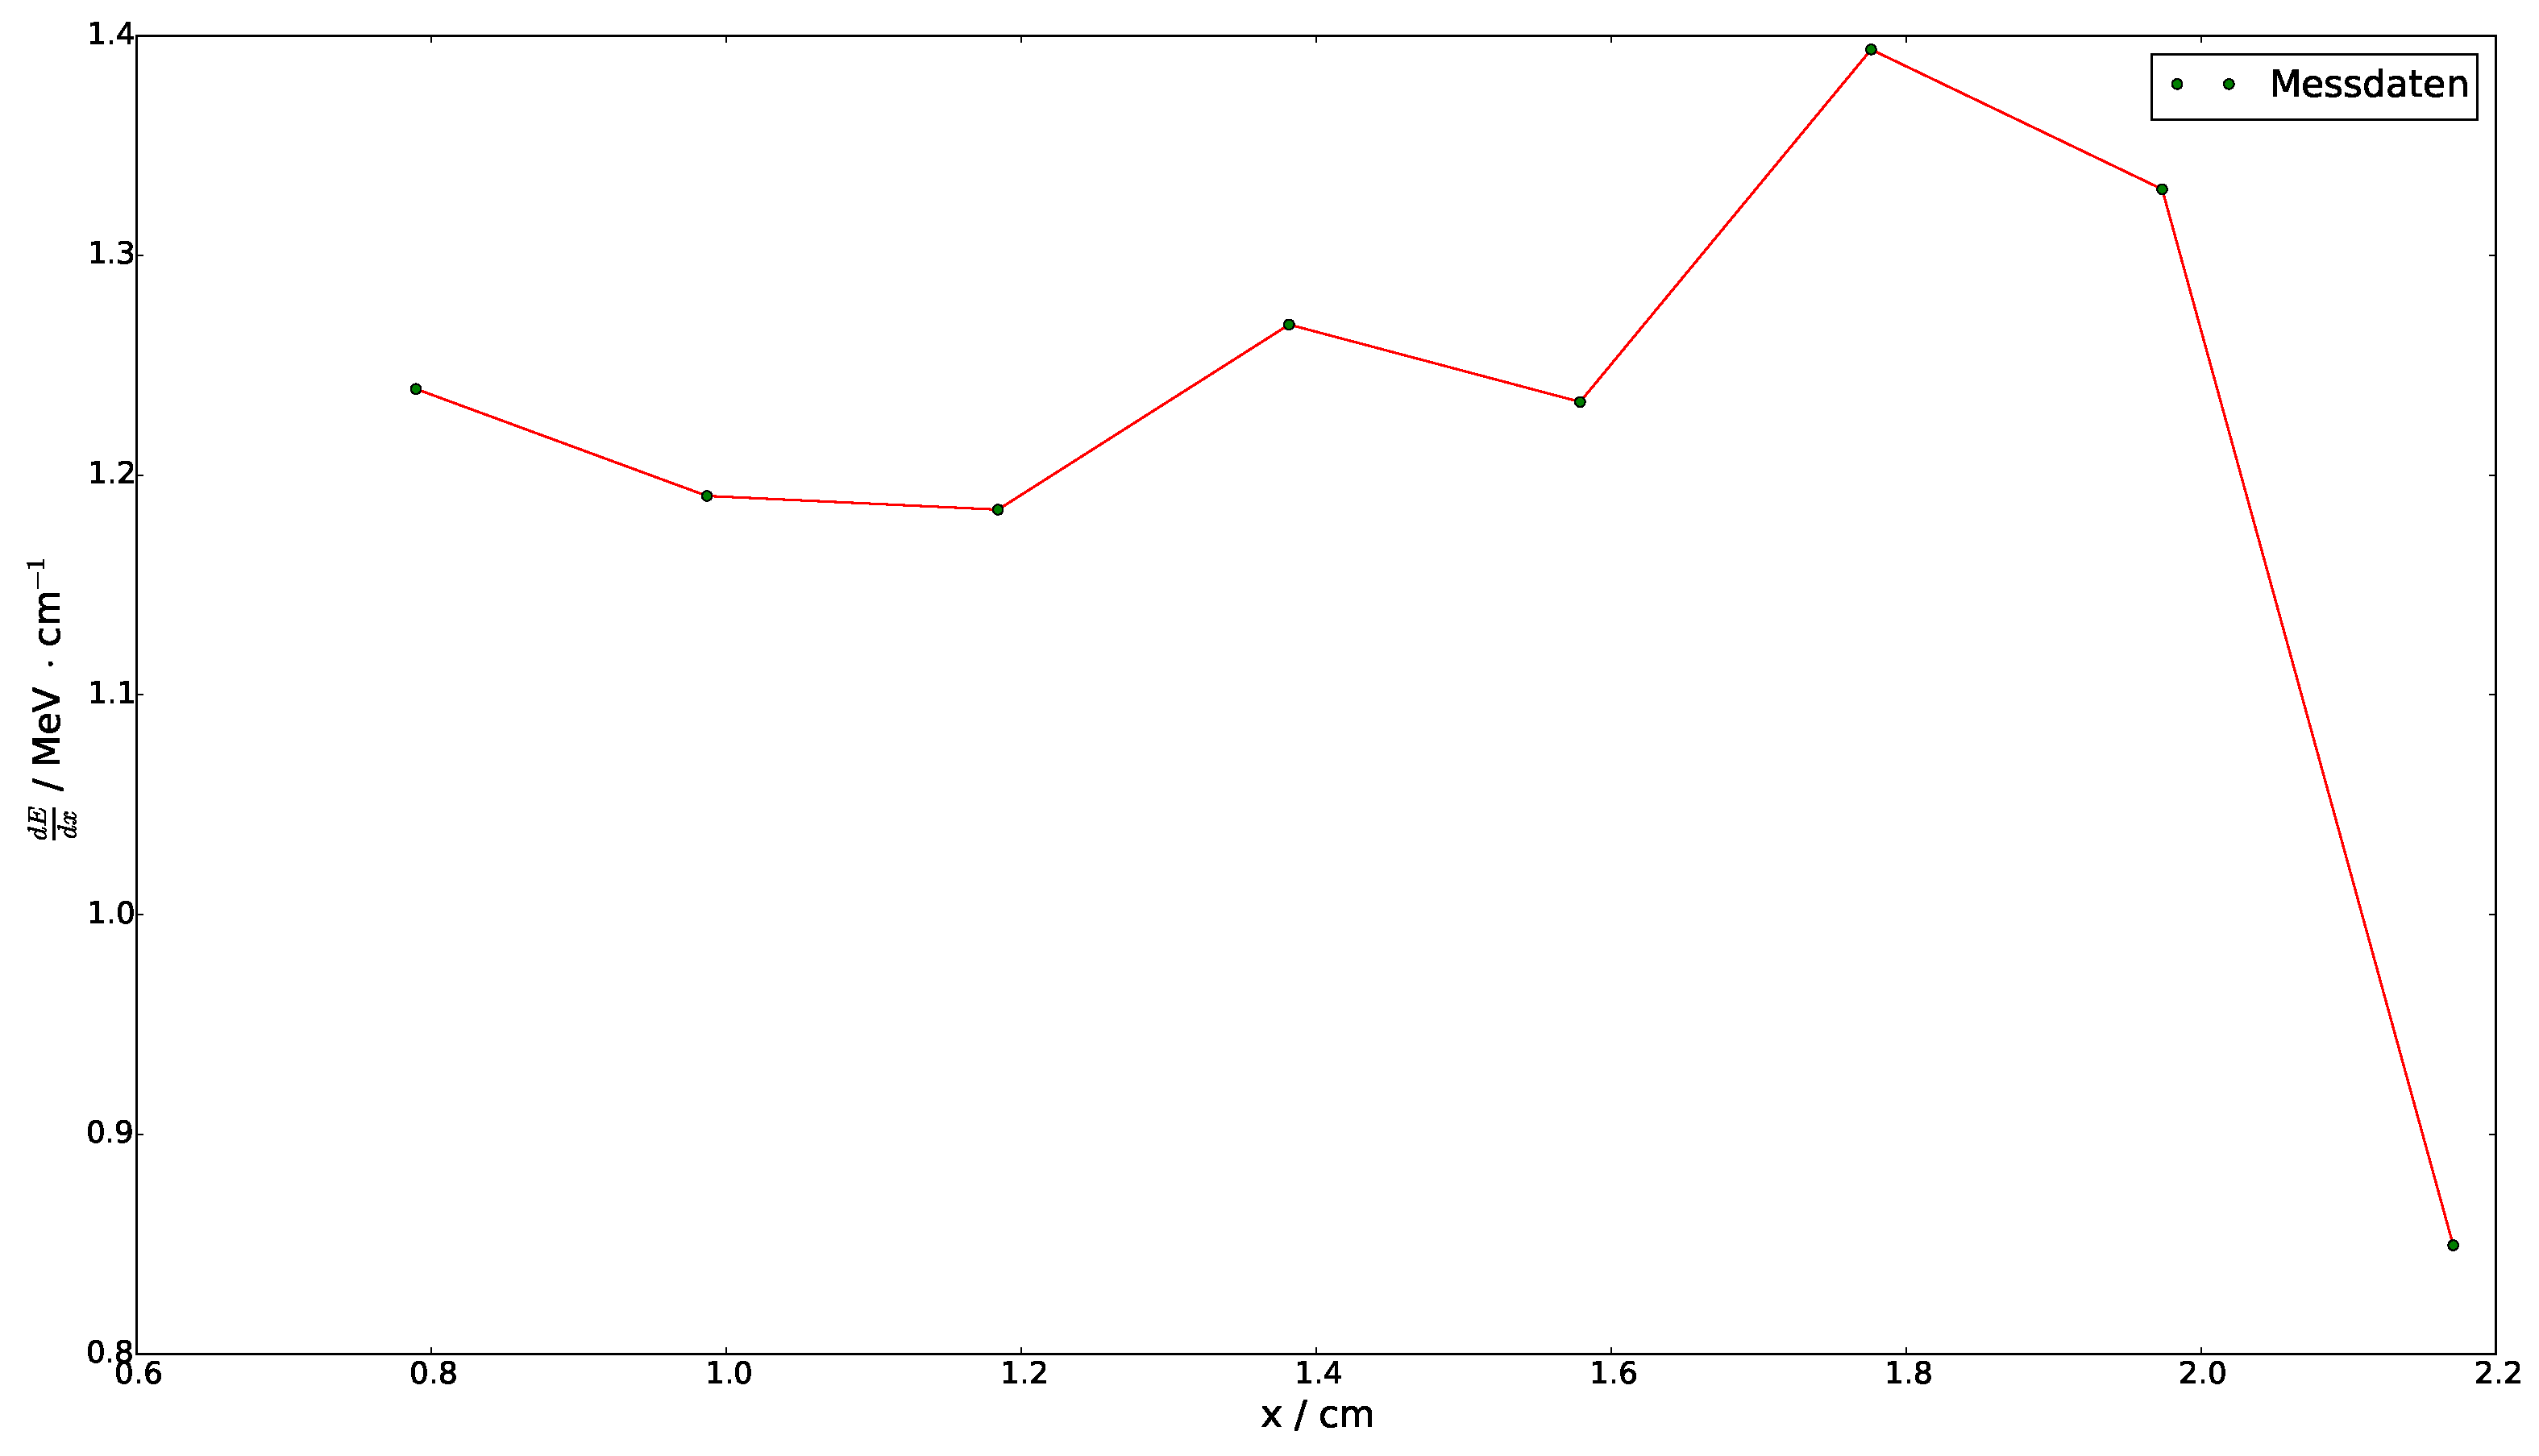
\includegraphics[scale=0.33]{bragg_kurve_2.pdf}
	\caption{$\frac{dE}{dx}$ gegen $x$ Aufgetragen ,der Braggpeak ist deutlich zu sehen}
	\label{fig:bragg_2}
\end{figure}

\noindent
In Abb. \ref{fig:bragg_3} ist f�r den 6 MeV Peak $\frac{dE}{dx}$ gegen $x$ zusehen.

\begin{figure}[H]
	\centering
  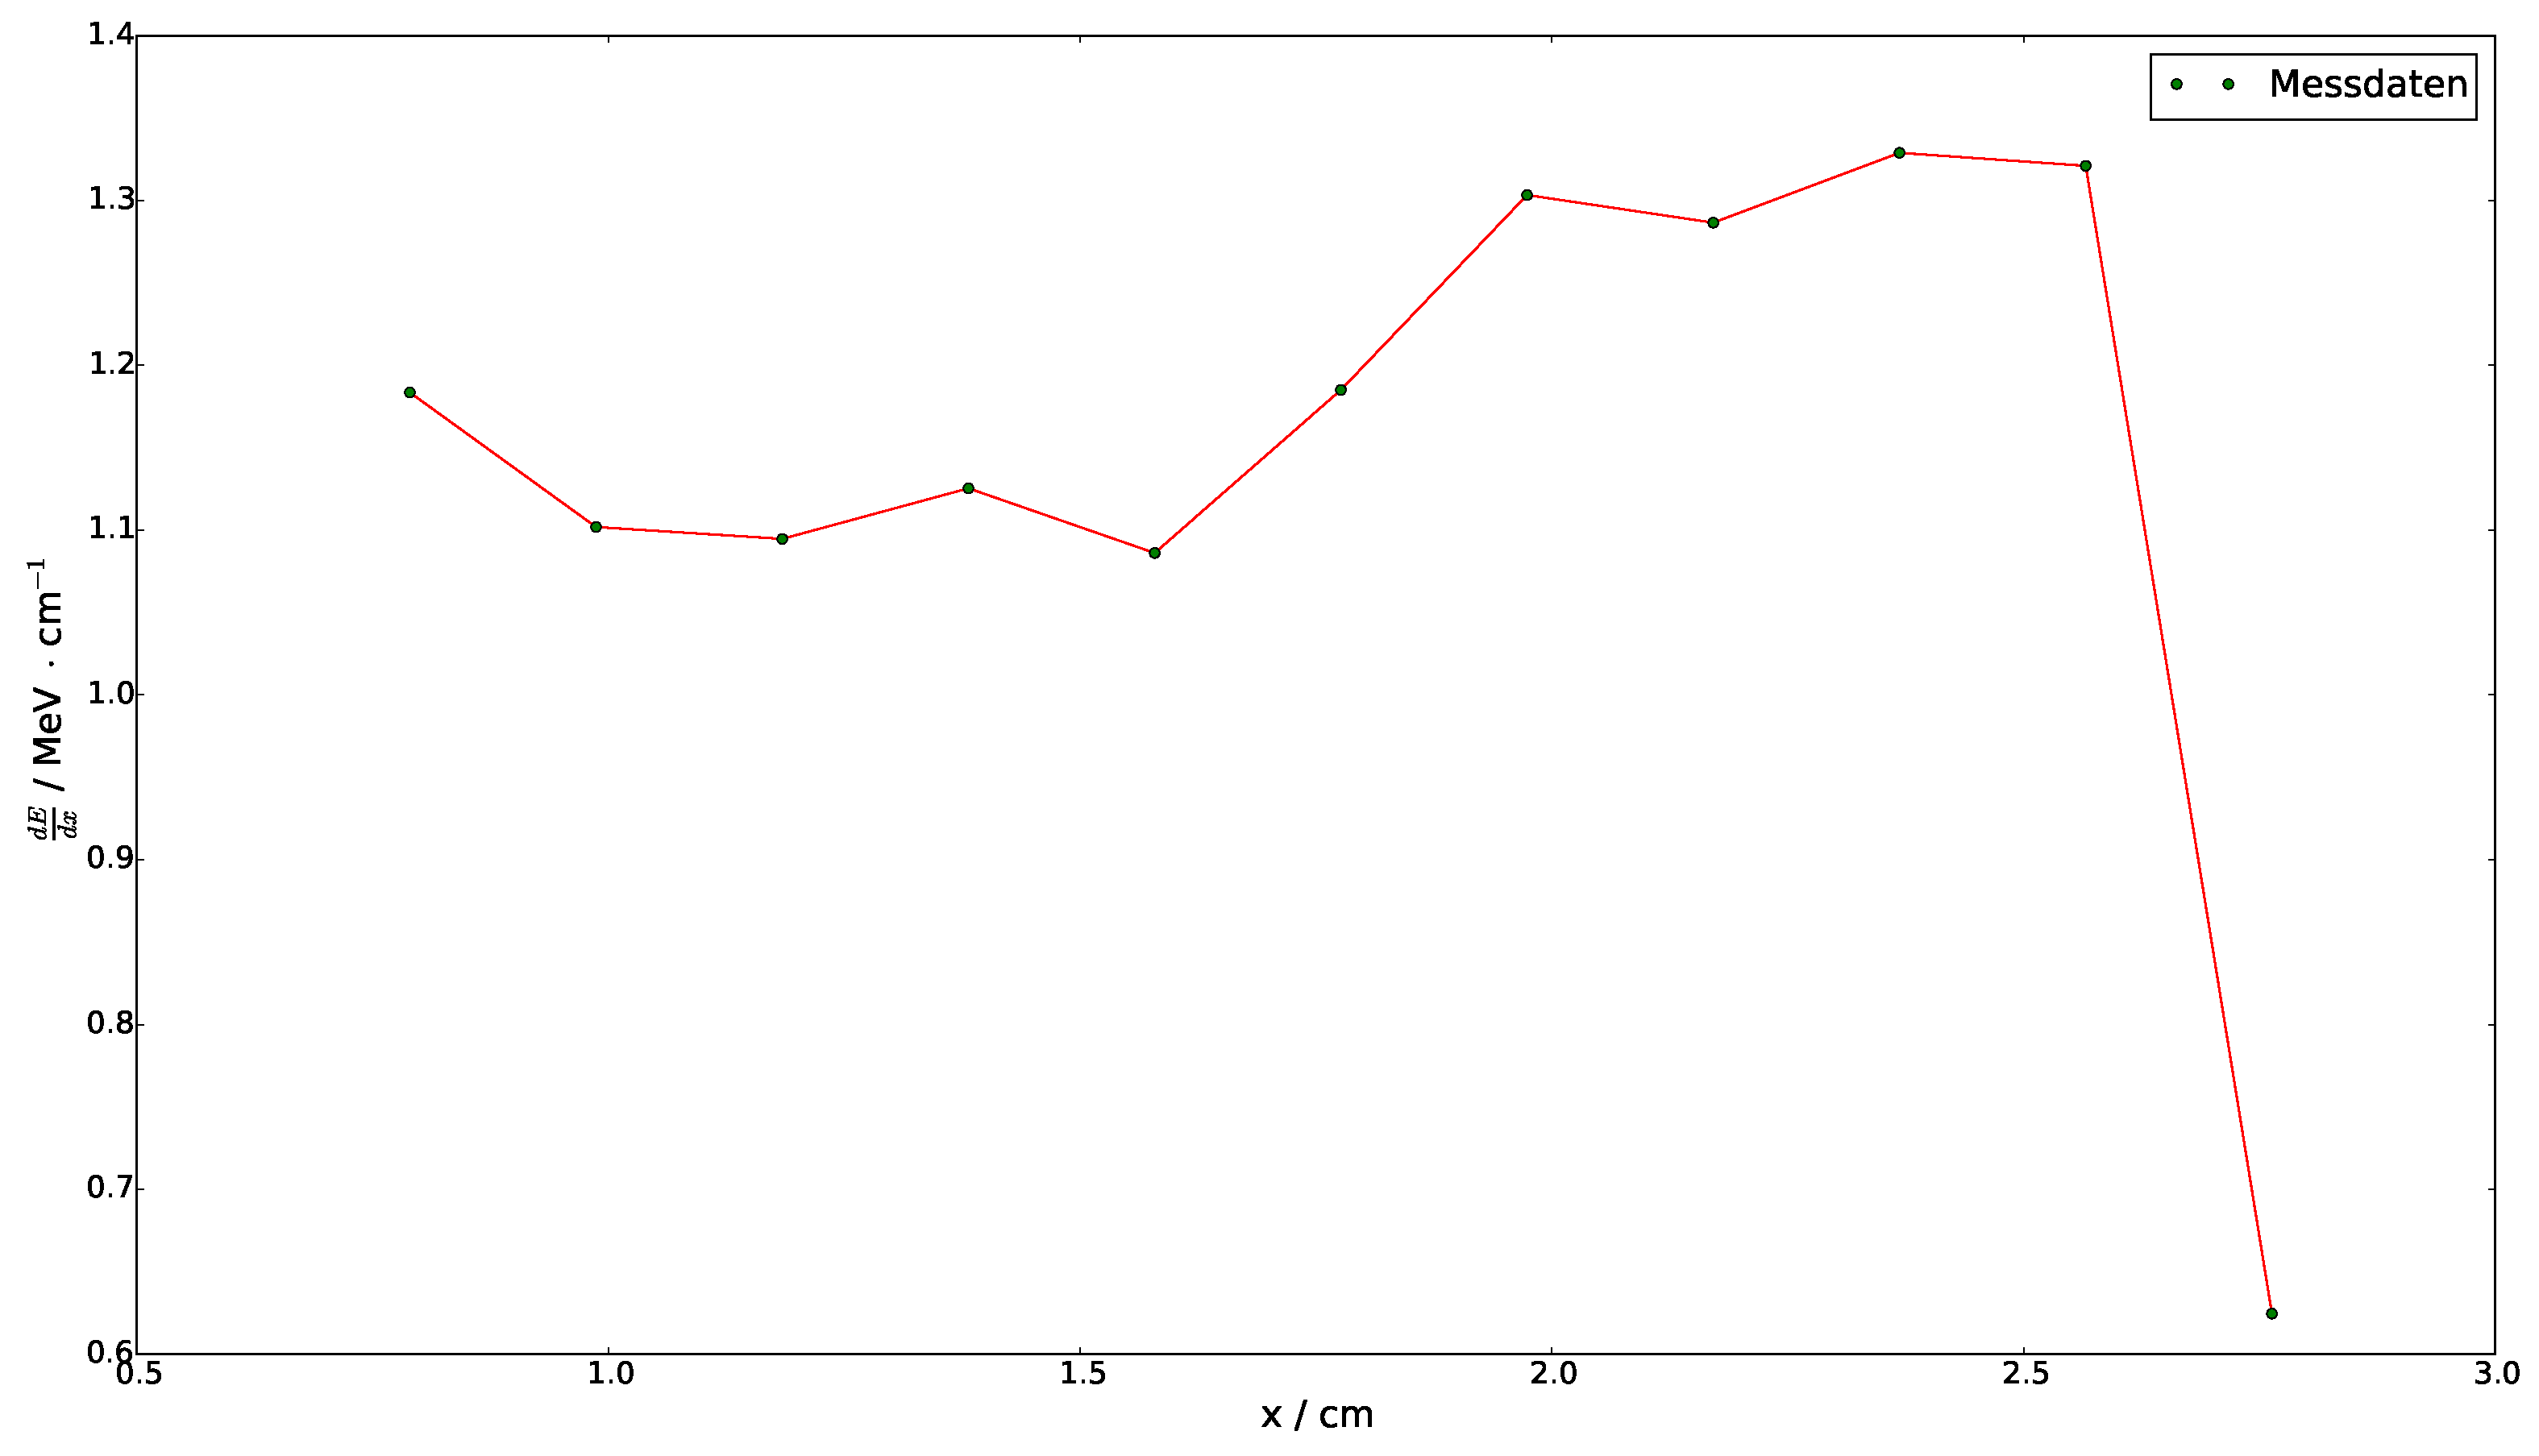
\includegraphics[scale=0.33]{bragg_kurve_3.pdf}
	\caption{$\frac{dE}{dx}$ gegen $x$ Aufgetragen , der Braggpeak ist gut sehen}
	\label{fig:bragg_3}
\end{figure}


\noindent
In Abb. \ref{fig:bragg_4} ist f�r den 7,69 MeV Peak $\frac{dE}{dx}$ gegen $x$ zusehen.

\begin{figure}[H]
	\centering
  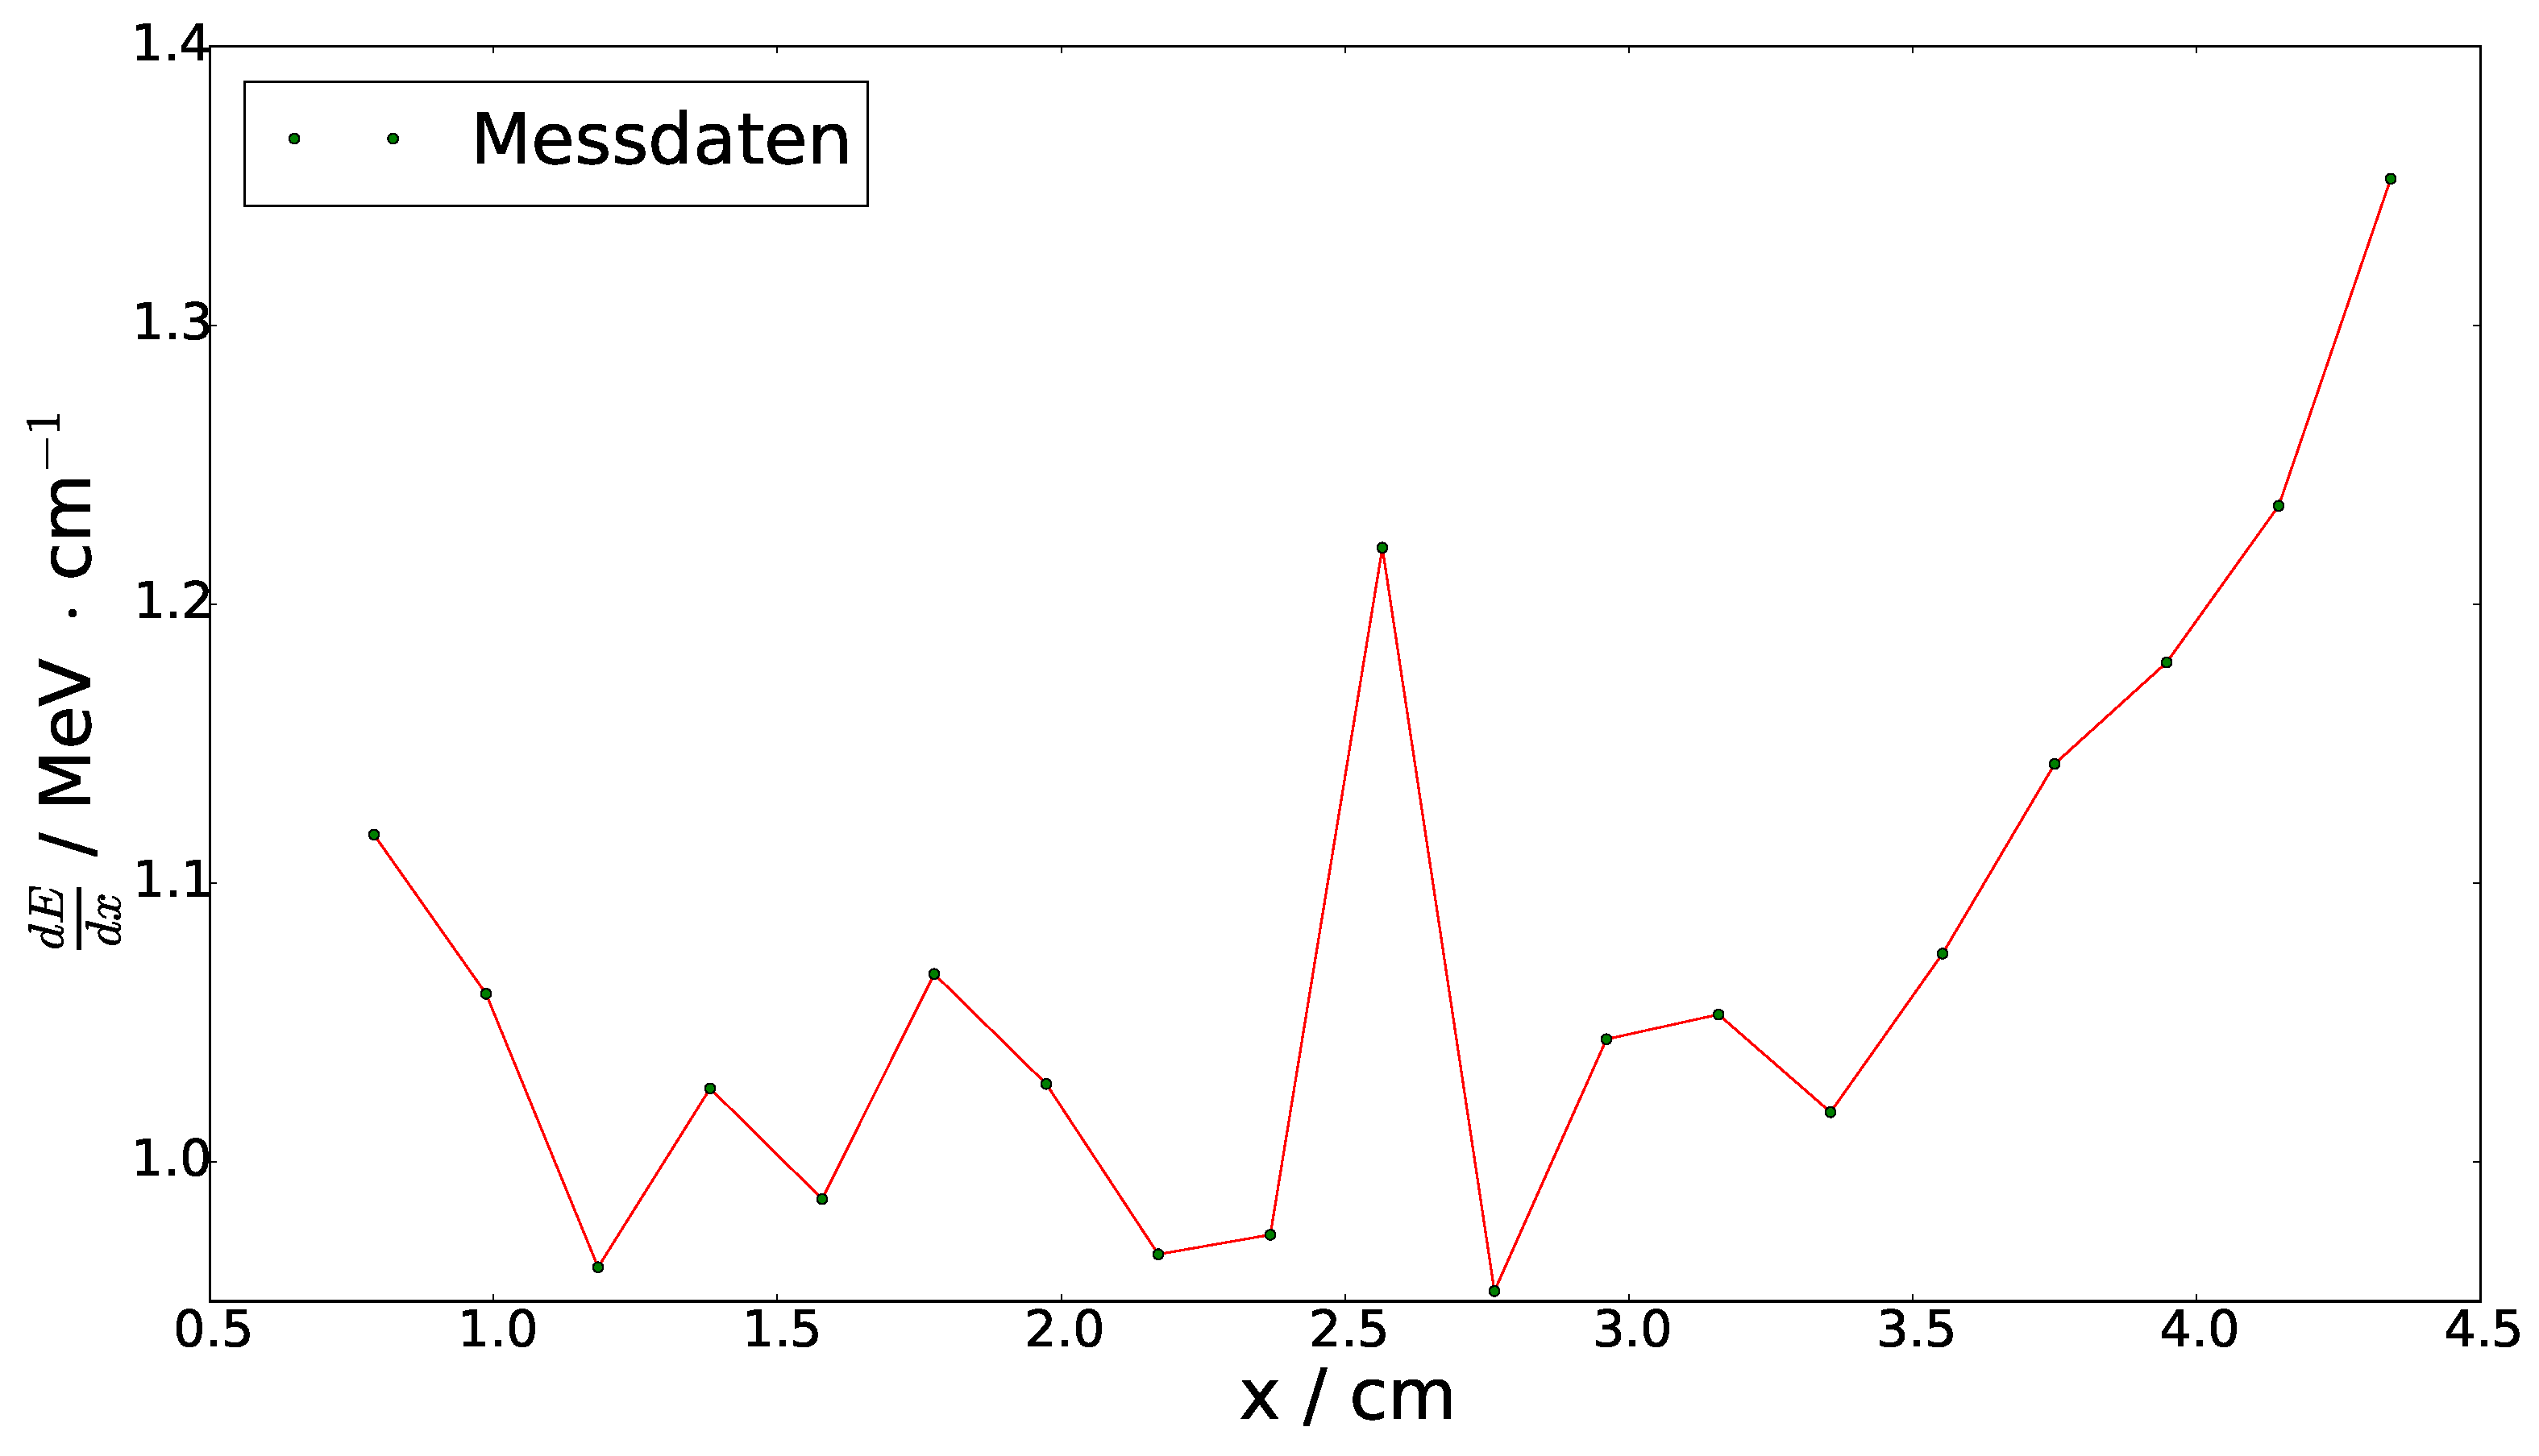
\includegraphics[scale=0.33]{bragg_kurve_4.pdf}
	\caption{$\frac{dE}{dx}$ gegen $x$ Aufgetragen , es Anfang des Braggpeaks ist deutlich zu sehen. Die Herkunft des Ausrei�ers bei ca. 2,5 cm ist nicht bekannt}
	\label{fig:bragg_4}
\end{figure}

Bei allen Plots ist die Form der Braggkurven zu erkennen. Vergleicht man die Abb. \ref{fig:braggkurve} mit Abb. \ref{fig:bragg_2}, so f�llt auf, dass der erwartete Peak bei 3,7 cm liegt, der Peak in Abb. \ref{fig:bragg_2} jedoch bei ca. 1.8 cm liegt. Woher die Schiebung kommt ist nicht bekannt.